\documentclass[10pt,twocolumn]{article}

% use the oxycomps style file
\usepackage{listings}
\usepackage{oxycomps}
\usepackage{appendix}
\usepackage{forest}
\usepackage{float} % Add this to your preamble
% usage: \fixme[comments describing issue]{text to be fixed}
% define \fixme as not doing anything special
\newcommand{\fixme}[2][]{#2}
% overwrite it so it shows up as red
\renewcommand{\fixme}[2][]{\textcolor{red}{#2}}
% overwrite it again so related text shows as footnotes
%\renewcommand{\fixme}[2][]{\textcolor{red}{#2\footnote{#1}}}

% read references.bib for the bibtex data
\bibliography{references}

% include metadata in the generated pdf file
\pdfinfo{
    /Title (The Occidental Computer Science Comprehensive Project: Goals, Timeline, Format, and Advice)
    /Author ( Alyanna McGrath)
}

% set the title and author information
\title{ \textit{What's on the Menu?} Transforming Occidental College's Menu Experience with a Full-Stack Solution
} % OxyEats: Redefining the Dining Landscape at Occidental College with an Interactive Marketplace Menu Web Platform
\author{Alyanna McGrath}
\affiliation{Occidental College}
\email{mcgratha@oxy.edu}

\begin{document}

\maketitle

\section{Introduction}

For college students living away from home for the first time, this transitional period becomes formative for eating habits. These habits often persist into adulthood and can significantly impact long-term health \cite{Norhaya2023}. Maintaining a balanced diet and knowing what’s available to eat on campus are essential components of a healthy lifestyle during these formative years. Yet, according to data from the American Time Use Survey (ATUS), full-time college students aged 18 to 24 dedicate an average of just one hour per day to ``eating and drinking" activities \cite{NewEngland2011}. This statistic highlights students' limited time to eat and drink, underscoring the importance of efficient digital dining solutions that fit seamlessly into their busy schedules. For many, balancing these demands while eating well is a persistent challenge. Time constraints, distance to the dining hall, and disorganized menus often make finding dining options difficult. Research by Burrows et al. (2017) underscores the link between dietary habits and academic performance, noting that planning meals around class schedules and extracurricular activities is one of the most time-consuming aspects of student life \cite{Burrows2017}. These factors highlight the pressing need for accessible digital menus that meet students' needs efficiently.
Doing so could significantly enhance students' daily experiences, both in terms of menu engagement and overall well-being.

\subsection{Problem Context}
These challenges are no different at Occidental College (‘Oxy’). Students need a convenient and efficient way to know what dining options are available, enabling them to make quick, informed decisions that fit seamlessly into their busy routines. The current digital menu solution for Occidental’s primary dining facility, the Marketplace—referred to in this paper as the ‘MP’—not only falls short in meeting students’ needs but only provides a basic, text-only display that lacks features to enhance the student experience. Other Southern California institutions with similar student populations and academic rigor have adopted interactive and visually engaging online dining menu systems that offer convenient accessibility and a user-friendly experience. By contrast, Oxy’s current menu platform remains limited in functionality; its interface is outdated, challenging to navigate, and less adaptable to students' daily needs. Additionally, there is a gap in how the Dining Department, particularly its administrative staff responsible for planning and updating menus, integrates student interactions (e.g., feedback, menu usage data) to inform menu decisions. This gap limits how effectively student feedback is integrated into creating new menus. Thousands of students interact with the menu site daily, presenting a missed opportunity to gather valuable data that could support dining staff in making more informed and evidence-driven decisions when planning menus. Further, for prospective students and visitors the outdated version reflects poorly on the college's commitment to providing a modern and accessible digital experience. Finally, as a senior with four years of firsthand experience navigating the frustrating menu system, I am driven to improve the overall experience by creating impactful, user-focused technology.

To address these issues, I propose a new interactive full-stack web application. The new solution will improve the menu display, making it more convenient, faster, and visually appealing. By leveraging advanced development techniques, the application introduces enhanced functionalities that improve students' overall user experience and provide dining staff with powerful management and data visualization tools.


\section{Technical Background}
I decided that this project should be in the form of a web application for two reasons. The first is that the current solution is a website. I did not want to diverge from that medium so that users did not have to learn something new. Additionally, given the project's time constraints of one semester, I decided to use a familiar process, as I have built web applications in the past.

A web application consists of a front end and a back end. For this project the frontend is written using ReactJS. The backend can be divided into two main parts: the server and the database. The server serves as the core component of the project, performing the scraping operation, and extracting menu item data from the original MP menu webpage. The database is essential for storing relevant information. I used GraphQL (a query language for APIs) for efficient data querying and manipulation and MongoDB as the database solution.


\subsection{MP Menu Ecosystem}
It is essential to grasp the current ecosystem to understand how my proposed solution will benefit both students and administrators in the dining department at Occidental. Insights were gathered through firsthand experience as a student and discussions with dining staff, including Robert Starec, Associate Director of Campus Dining, and Nathan Martinez, Director of Culinary Services. Martinez joined Occidental five months ago from the University of Southern California (USC). Martinez, has spent his first months understanding existing processes and challenges. The dining department operates a complex ecosystem grounded in a five-week cycle menu see Fig.\ref{mp-ecosystem}. The process outlined in this figure illustrates the key steps, from menu planning to incorporating feedback for continuous improvement.

    \begin{figure}[htbp]
    \centering
    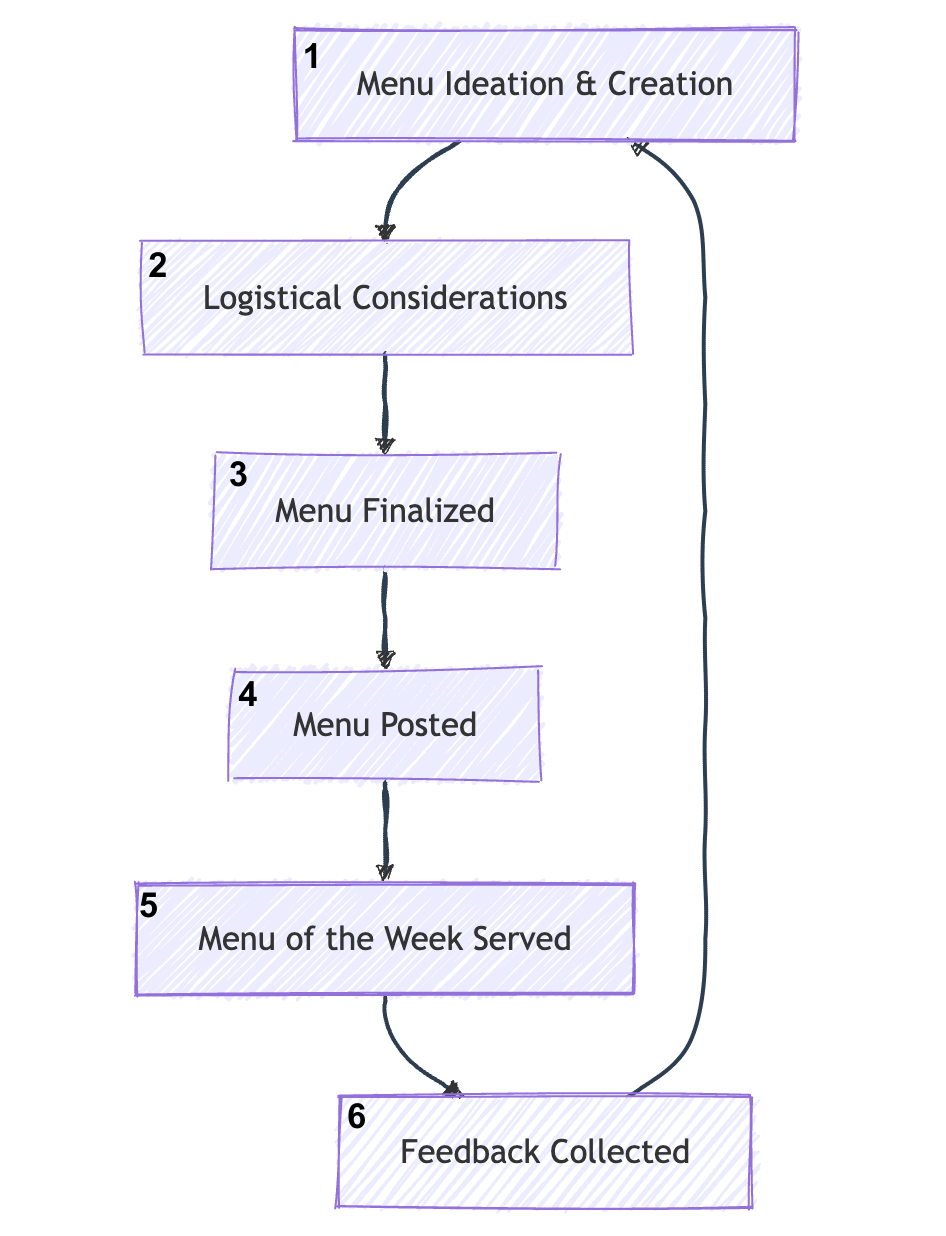
\includegraphics[width=.55\linewidth]{images/mp-ecosystem.png} % Adjusted width
    \caption{
        The ecosystem visualized as a flowchart
    }\label{mp-ecosystem}
\end{figure}


 

\begin{enumerate}
    \item \textbf{Menu Ideation and Creation}: This process begins with menu planning, where the culinary team generates ideas for the meals they want to serve.
    \item \textbf{Logistics}: With a shortlist of ideated meals in mind, the team begins factoring in essential logistics, such as inventory of available ingredients, budget constraints, and ordering supplies. They also consider seasonal availability while ensuring variety, nutritional balance, and meals that appeal to student preferences. 
     \item \textbf{Menu Finalized}: The finalized menu is stored in an archive, which consists of a comprehensive Excel spreadsheet listing meal items, their ingredients, and other relevant information.
     \item \textbf{Menu Posted}: The weekly menu is manually typed into the MP menu website on the Sunday before the start of the week. Unlike a web app (the medium of my proposed solution), which offers interactive features and functionalities to engage users, the MP menu website is strictly a static website that displays information.  The website is nested within the home page, requiring navigation through multiple tabs. The navigation path is as follows: Home → Student Life → Campus Dining → Where To Eat → Marketplace. The menu is presented weekly, displaying all seven days on a single page. It should be noted that the webpage is not responsive to mobile devices, meaning it is less user-friendly on a cellphone compared to a laptop due to the excessive scrolling required to navigate.
   \item \textbf{Menu Served}: As the title suggests, the meals planned for that week are prepared and served to students.
      \item \textbf{Feedback Collected}:  Finally, before the cycle repeats, the dining department integrates feedback into its planning process to ensure continuous improvement. According to Martinez, quantitative feedback is key to evaluating a meal's success. The department uses a Point-of-Sale (POS) system powered by Oracle to track sales data; by analyzing the data, a benchmark of 300 servings or more per meal period generally indicates a meal's relative success. Meal periods refer to breakfast, lunch, and dinner, while stations include Homestyle, Sauté, Grill, and Chef's Corner. Additionally, the department gathers feedback through a public 'Suggestion Form,' located on a separate subpage of the main website (Home → Student Life → Campus Dining). This form addresses the entire dining experience at Occidental College. While not specific to the MP, any comments about meal items are reviewed and factored into future planning. Another informal feedback method involves monitoring food waste. Though there is no standardized tracking system, dining staff monitor food waste by observing leftover food on plates at the drop-off conveyor and comparing trays of prepared but untouched food to the quantities initially served. This provides valuable yet inconsistent insight into the success of meals and opportunities for improvement.
\end{enumerate}

Outside the described ecosystem, updates or announcements related to the menu or the Marketplace (MP) operate through separate, compartmentalized systems. For instance, the daily menu is posted both on the webpage and on Instagram Stories, highlighting each meal area for the two primary dining times: lunch and dinner. Daily updates, announcements, or special meals are also shared on Instagram. However, this platform has a limited reach, with approximately 880 followers, and does not encompass the entire student body. For broader announcements, such as special MP hours during holidays or theme-based menus, dining staff rely on email communications through the Student Digest sent to all students.

Several inefficiencies exist in this ecosystem. Menu management, POS data analysis, and feedback intake are handled by separate teams with minimal integration. The department relies heavily on Excel spreadsheets to manage operations, further highlighting the fragmentation. The lack of a unified platform has prompted the department to explore consolidation efforts, with CBORD (a backend menu management platform) positioned as a potential integrator. However, the implementation of CBORD is still in progress, with no clear timeline for full functionality. This gap presents an opportunity for my full-stack web application to centralize data and streamline team communication. In addition, the student feedback process needs significant improvement. The feedback form is not easily discoverable, and, according to Director Martinez, it is rarely used to submit positive comments or praise for meals. Most submissions focus on dissatisfaction. Martinez often has to actively prompt students for feedback by engaging with diners in MP or in passing around campus, to share positive feedback or confirm whether they enjoyed a specific meal item. This underscores the need for a more effective and accessible feedback mechanism as part of a broader technological solution. As Martinez observed during his short time at Oxy, the dining department struggles with integrating technical systems compared to his tenure at USC, largely due to IT processes and the extensive steps required for system approvals. A striking example is the delayed implementation of a credit card payment system for non-students, highlighting the department's slow adoption of modern solutions. My proposed solution aims to address steps \#4 and \#6 of the ecosystem by streamlining how menus are posted and integrating feedback into the decision-making process through a unified, user-friendly platform.

\subsection{User Experience and Usability}
In developing and evaluating the proposed web application, a strong emphasis is placed on both usability and user experience (UX). As defined by the International Organization for Standardization (ISO 9241-11), usability refers to the effectiveness, efficiency, and satisfaction with which specific users can achieve their goals in a particular environment \cite{ISO2018}. User experience extends beyond this, encompassing users' overall perceptions and responses during interaction with the system, including emotional, cognitive, and physical reactions. A comparative study of UI design tools—Sketch, Adobe XD, and Figma—revealed that Figma outperformed the others in usability and UX due to superior interface layout, information quality, and interaction logic \cite{UX2022}. The research emphasizes that while usability ensures functionality and efficiency, the user experience determines emotional engagement and satisfaction that ultimately drive adoption and sustained use \cite{UX2022}. With my project, I aim to enhance usability by ensuring accurate and current menu information, a user-friendly interface that provides a delightful student experience, and a streamlined management and feedback viewing experience for administrators (UX). In doing so, the project addresses key gaps in the MP menu ecosystem.

\section{Prior Work}
\subsection{ Research on the Format of Restaurant Online Menus}
While college dining halls and traditional restaurants serve distinct audiences, they share similarities in delivering meals and user experiences. Online menus, a critical touchpoint for both, play a significant role in shaping user experiences. Although there is not a considerable body of literature on college dining menu design, insights from restaurant menu design strategies can inform improvements to institutional dining systems, better addressing the needs of Occidental’s students and faculty.

Prior research suggests that effective menu design is critical in enhancing user experience and driving engagement. The study by Kateryna Fedosova, ``Development of an Effective Restaurant Menu: Research and Recommendations" explores menu design's psychological and structural aspects to optimize both consumer choices and profitability. The study results show that grouping items logically, such as by type (e.g. drinks, sides, sandwiches, etc) or ingredients, significantly enhances menu navigability and reduces cognitive overload. This aligns with findings from neuromarketing studies emphasizing the ``paradox of choice," where excessive options can overwhelm customers, ultimately leading to decision fatigue and preference for familiar items \cite{Fedosova2022}. For example, the study highlights that smaller menus, featuring 3–7 items per group are more effective in guiding user choices than expansive, unstructured menus.
Additionally,  research shows that strategically positioning high-margin items in the top-right corner or center of the menu—areas where consumers' eyes are naturally drawn first—can maximize sales. This was successfully established as described by the implementation at BLOOM Cafe, which reported a 15.8(percent) increase in sales after redesigning its menu based on these principles \cite{Fedosova2022}.
A recent study, ``The Effect of Online Restaurant Menus on Consumers’ Purchase Intentions During the COVID-19 Pandemic," supports these ideas by using the Stimulus-Organism-Response (S-O-R) model to explore how menu design affects customer behavior. The study found that visually appealing menus, with clear layouts and attractive images, grab people’s attention and make them feel more positive about the food \cite{Covid2021}. This emotional connection increases their interest and makes them more likely to choose and purchase items. Together, these features create a better overall experience and encourage more engagement with the menu. 

Insights from restaurant menu design, such as grouping items logically to reduce cognitive overload, directly shape this project's approach to improving Oxy’s menu navigation, making it easier for students to find meals. While the research highlights the impact of visual imagery in restaurants, this is less relevant for college dining due to frequently changing menus and the challenge of creating new images for daily meal items across multiple dining periods. This project focuses on real-time updates to show current meal options and clear textual descriptions to help students make quick, informed decisions. Unlike restaurant menus designed to maximize sales by emphasizing high-profit items, this is irrelevant to a residential academic institution like Occidental, where the focus should be on priorxitizing student satisfaction and accessibility. By adopting only the relevant principles from restaurant menu design, this project addresses the unique needs of a student-focused dining system.

\subsection{ Exemplary solutions}

I conducted an in-depth comparative analysis of dining menu webpages across schools in the Southern California Intercollegiate Athletic Conference (SCIAC) to identify trends and functionalities that inform this project’s design. SCIAC includes 12 colleges with shared characteristics, such as similar institutional size, geographic proximity, and high academic standards, making them valuable benchmarks. Among the 12 colleges in the Southern California Intercollegiate Athletic Conference (SCIAC), eight schools utilize third-party dining services like Sodexo or Café Bon Appétit, which standardize features such as allergen filtering, dropdown navigation, and live operational updates. By being able to access all information in one place, students can quickly determine if the dining hall is open, view what is being served, and efficiently refine meal options based on their dietary needs, making the dining process more convenient and user-friendly. Ten colleges offer a default navigation system that displays the current day’s menu upon accessing the page, making it easy for users to focus on immediate meal options. In contrast, Oxy is the only institution that only provides a full week’s menu on a single page, offering a broader overview but potentially overwhelming users seeking specific daily information.

Nutritional transparency is another significant strength, with nine schools offering some or all of the following: detailed macronutrient information, calorie counts, allergen details, and ingredient lists. However, integrating nutritional labeling into this project is not feasible due to resource and time constraints. Director Martinez noted that adding nutritional details is not a top priority, as it would require staff oversight, which is unrealistic given their already stretched capacity. Instead, the department opts to post dietary labeling for meals physically in the MP rather than online. Considering that, the project will focus on addressing navigation and real-time usability gaps, which are more pressing for enhancing student experiences. A full comparative table of eleven SCIAC schools, excluding Caltech, as its dining menu was not accessible to non-students, can be found in Appendix \ref{appendix-test}.

\subsubsection{Uber Eats and Google}
    \begin{figure} [H]
    \centering
    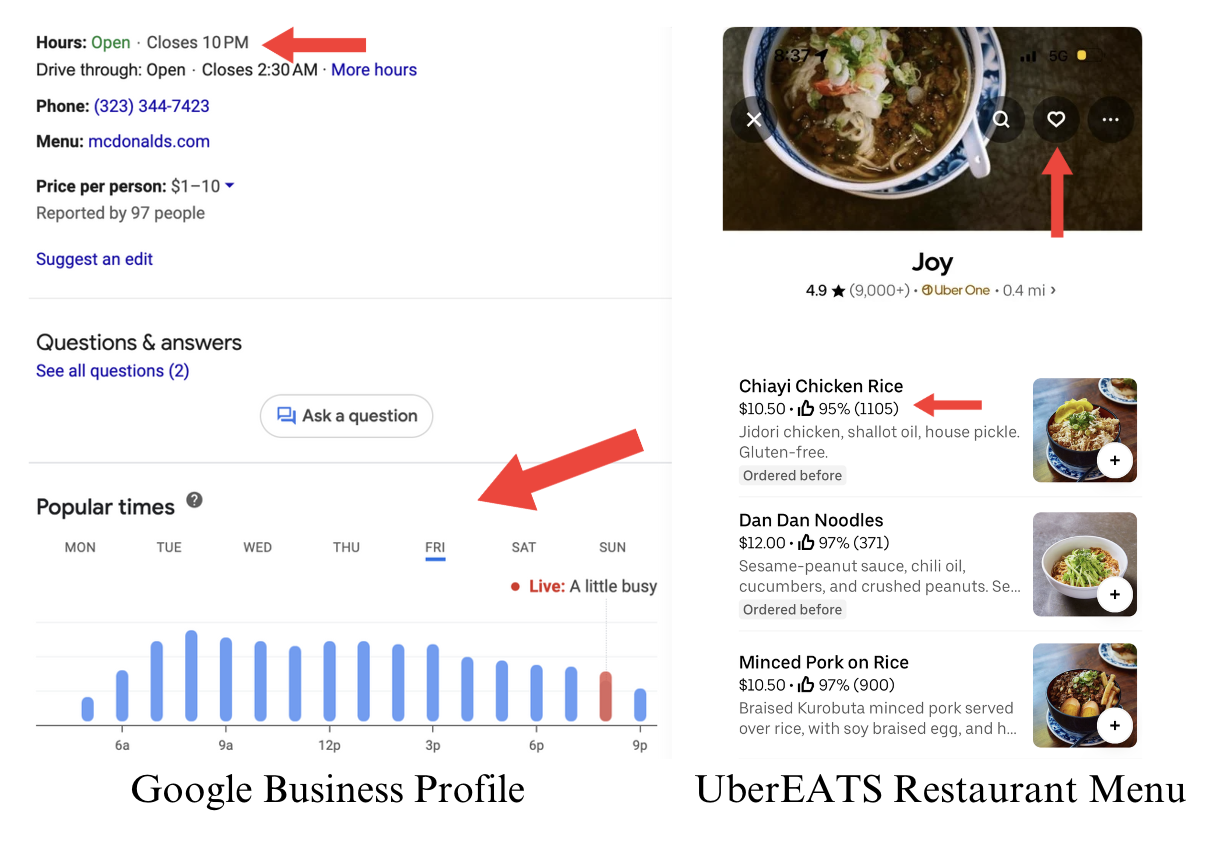
\includegraphics[width=.95\linewidth]{images/ubereats.png} % Adjusted width
    \caption{
        Exemplary solutions by popular services
    }\label{uberEATS}
\end{figure}
Building on insights from SCIAC dining platforms, food delivery systems like Uber Eats showcase efficient, user-friendly design principles that inspire the application design. As shown in Fig. \ref{uberEATS}, social ratings (e.g., the percentage of users who ‘thumbs-upped’ a meal and the number of feedback submissions) provide dual benefits: helping restaurants understand item popularity while guiding customer decisions by highlighting well-liked options. Uber Eats also allows customers to “favorite” and save restaurants for quick access, emphasizing personalization and convenience. Similarly, Google Business Profiles, shown on the left of Fig. \ref{uberEATS}, improve usability by displaying essential information, such as live status (open or closed) and busyness levels, in a concise format. This streamlined approach ensures users can quickly access the details they need without navigating multiple pages, enhancing convenience and efficiency. The favoriting and rating systems on Uber Eats especially influence the potential for personalization in this project, allowing users to save preferred meals and provide feedback that can also inform dining staff for menu planning and improvements. None of the SCIAC schools provide advanced personalization features, highlighting an opportunity for innovation. This project aims to incorporate tools such as meal saving and rating to enhance user interaction and support feedback for dining staff. 

\section{Methods}

In creating this web application, I relied heavily on the research-backed advice and processes outlined in a respected, comprehensive design manual, Web Style Guide \cite{Web2009}. The book's principles remain highly relevant despite being over a decade old. According to the Association for Computer Machinery (ACM), the guide offers valuable insights into designing for accessibility, maintaining websites, and using style sheets developed by Yale University’s Center for Advanced Instructional Media.
The development of this application followed a classic software design life cycle (SDLC). I followed the waterfall method, completing each phase sequentially before moving to the next. However, I adopted an iterative approach during the testing phase, incorporating user feedback to improve the application. A visual representation of the Waterfall SDLC is provided in Appendix \ref{waterfall-sldc}.

\subsection{Requirements}
The first step in any web design process is to understand the users—who they are, their goals, and their needs for interacting with the site. This initial research phase is critical for creating a user-focused solution \cite{Web2009}.  For my project, all participants in the user interviews, testing sessions, and survey completion were incentivized through a \$50 Amazon gift card raffle.

\subsubsection{Initial Interviews (Students)}
I planned a series of initial virtual interviews to achieve two key goals: understanding students’ current sentiments about the MP webpage and observing their behaviors and interactions with the existing platform. I consulted the UXR Field Guide to learn how to craft non-leading, open-ended questions, ensuring that I would gather unbiased and genuine feedback \cite{UXR}. I also sought guidance from a CS professor with expertise in human-computer interaction, who provided feedback on effectively structuring the Zoom interviews.  The interviews included 16 students, including five first-years, four sophomores, five juniors, and two seniors. The interview was split into two parts: first, participants shared their screens, navigated the MP website, and commented on their actions while I observed silently. The second part involved direct, focused questions based on my observations. In a short pre-testing demographic questionnaire most participants (75\%) reported using the webpage multiple times a week, with many checking it daily for meal planning, dietary information, or to confirm dining hours and locations. 

From the virtual interviews, I noticed a pattern of things across behaviors with the sites; it was evenly split between students who used the jump-to-day functionality or just scrolled to the day. Students who scrolled to the day almost always missed the day they were looking for, scrolling past it or scrolling too short. Also, navigating to the menu, I noticed that most students typed in 'Market' into the search bar, and the URL would autofill. Only about two to three students navigated to the dining homepage and clicked through subpages to get to the menu. Positive feedback focused on the clarity of the existing layout, with students appreciating the hyperlinks at the top of the page for navigating daily menus. Bolded days were also mentioned as valuable elements of the design. Despite these strengths, the interviews revealed several consistent pain points. Over half of the participants noted that the webpage is often not updated promptly, leading to frustration when meal options are outdated or missing. While this is valuable feedback, it is less relevant to my project, as the menu data will be scraped directly from the original webpage. However, this highlights the importance of ensuring that the network and loading speeds of the new platform are sufficient to emphasize user convenience. All students also criticized the font style choices, citing difficulty in differentiating between meal stations and food items due to the uniformity of the text formatting. Student suggestions to enhance the layout included increasing the spacing between days and sections and using visual differentiation, such as bolding or italics, to make meal station headings more prominent. 

These findings highlight consistent dissatisfaction with the lack of dietary labeling, outdated menus, and confusing layouts while recognizing the strengths of the current navigation structure. This feedback directly informs the project’s design priorities, emphasizing improved accessibility, timely updates, and enhanced visual organization to better meet student needs.
\subsubsection{Initial Survey (Students)}

After completing the Zoom interviews, I summarized key findings and created a survey to gather quantitative data on student satisfaction with the current MP menu webpage. The survey also identified features students were most excited about and helped shortlist participants for future user testing.The survey covered topics such as user satisfaction, ease of navigation, layout and formatting, and desired features. Definitions for terms like “layout and design” and “difficulties” ensured participants shared a clear understanding of the questions, leading to accurate responses.The survey included Zoom interview participants and seven additional students, totaling 23: seven first-years, seven sophomores, four juniors, and five seniors. For the discussed ratings (unless otherwise noted), all averages were based on a five-point Likert scale. Students rated navigation ease at an average of 3.78, citing uniform text styles that made sections hard to distinguish. While they appreciated the hyperlinks at the top, many found the layout “cluttered” and unorganized. Participants described the menu as plain and unengaging, suggesting improvements like a more visually appealing design and a chart or table format for easier navigation. Top requested features included dietary restriction filtering, weekly email notifications, a menu item rating system, and a quick link search feature for unfamiliar items. Overall satisfaction averaged 6.96 out of 10, with only three students rating it above 9 and eight rating it five or below, indicating significant room for improvement. These responses highlight key areas for enhancement and guide feature development to align with student needs. A file containing the raw survey data is available in the GitHub repository, located in the .FinalPaper/assets directory under 'Initial MP Survey' \cite{GitHubRepo}.

\subsubsection{Understanding Admin Needs}
 I brought the preliminary findings from the survey and initial interviews to the dining department for review and discussion. Informally, I spoke with staff members during visits to the MP, gathering insights on challenges like managing menu updates and collecting student feedback. One key takeaway from these conversations was their desire for better communication tools to engage with students. This was further emphasized during formal meetings with dining department administrators, including Director Martinez, who highlighted his interest in announcing new menu items and encouraging students to complete feedback forms. These discussions underscored the importance of features like live announcements and streamlined communication within the admin interface. By incorporating these insights, I ensured the project aligned with both the staff’s operational needs and their goals for improved student interaction.

\subsubsection{Finalizing Requirements}
After completing the interviews and analyzing the survey results, I could now define the use cases alongside my research on exemplary solutions and practical design principles. The phrase 'use case' refers to specific scenarios in which an user interacts with the system to achieve a goal. These requirements are categorized into three user groups: a casual user—anyone who visits the page; a student user—a student logged in to the system; and an admin user—a dining department administrator managing the backend. Casual users and student users are not mutually exclusive. 
I have written AAU (As A User) statements for each requirement to ensure clarity and user-centered focus. This is a widely adopted practice in Agile software development. This methodology emphasizes understanding and addressing user needs, ensuring each feature delivers tangible value \cite{AAU}. 

As a \textbf{Casual User}:\vspace{-1em}
\begin{itemize}
   \item  I want to view today’s menu quickly and easily distinguish between different meal items
    \item I want to filter meal items to identify options that meet my dietary preferences or restrictions
    \item I want to browse the menu on my mobile device efficiently
    \item I want to know the live status of the MP (open/closed) and its current hours
\end{itemize}
As a \textbf{Student User}:\vspace{-1em}
\begin{itemize}
   \item I want to rate meal items I’ve eaten to reference them later and provide feedback to the dining staff
    \item I want to save meal items to a favorites list for easy reference in the future
    \item I want to receive the weekly menu in my inbox at the start of each week
    \item I want to provide open-ended feedback easily on the same page where I view the menu
\end{itemize}
As an \textbf{Admin User}:\vspace{-1em}
\begin{itemize}
   \item I want to see the performance of meal items based on ratings and favorites to make informed decisions
    \item I want to update the menu and meal items in the system quickly
    \item I want to set pop-up announcements for students to see dynamically
    \item I want to view student responses to open-ended feedback within the same system
    \item I want to easily manage and adjust the MP’s operating hours
\end{itemize}

\subsection{Interface Design}
The next step in the SDLC is to apply what is learned in the research phase to create designs \cite{Web2009} . Building on the insights gathered from the requirements phase, the design phase focused on creating mockups that addressed the specific user needs. Traditionally, especially for a web-based solution, designs start as wireframes and then prototypes and are finally transformed into functional mockups. Due to time constraints, I prioritized paper prototypes for quick feedback and easy revisions without extensive design work. In creating these mock-ups, I relied on my intuition and creative skills to envision how the webpage should look while drawing inspiration from exemplary website solutions and best practices in menu design. I equally prioritized aligning the designs with Universal Design principles developed by the Center for Universal Design at North Carolina State University, which are particularly relevant to web environments.
\vspace{-1em}
\begin{enumerate}
   \item \textbf{Equitable Use}: Designs should work for all users, providing identical or equivalent ways to interact, offering flexibility not possible in physical formats \cite{Web2009}.
    \item \textbf{Flexibility in Use}: Designs should accommodate different preferences and abilities. Web users can adjust settings, such as disabling images or changing layouts and fonts, to suit their needs \cite{Web2009}.
    \item \textbf{Simple and Intuitive Use}: Designs should eliminate unnecessary complexity, presenting information clearly and organized. For web design, simplicity and direct access to essential features improve usability \cite{Web2009}.
    \item \textbf{Perceptible Information}: Necessary information should be accessible to users regardless of their sensory abilities, ensuring compatibility with assistive technologies \cite{Web2009}
\end{enumerate}

\subsubsection{Prototypes}

    \begin{figure}
    \centering
    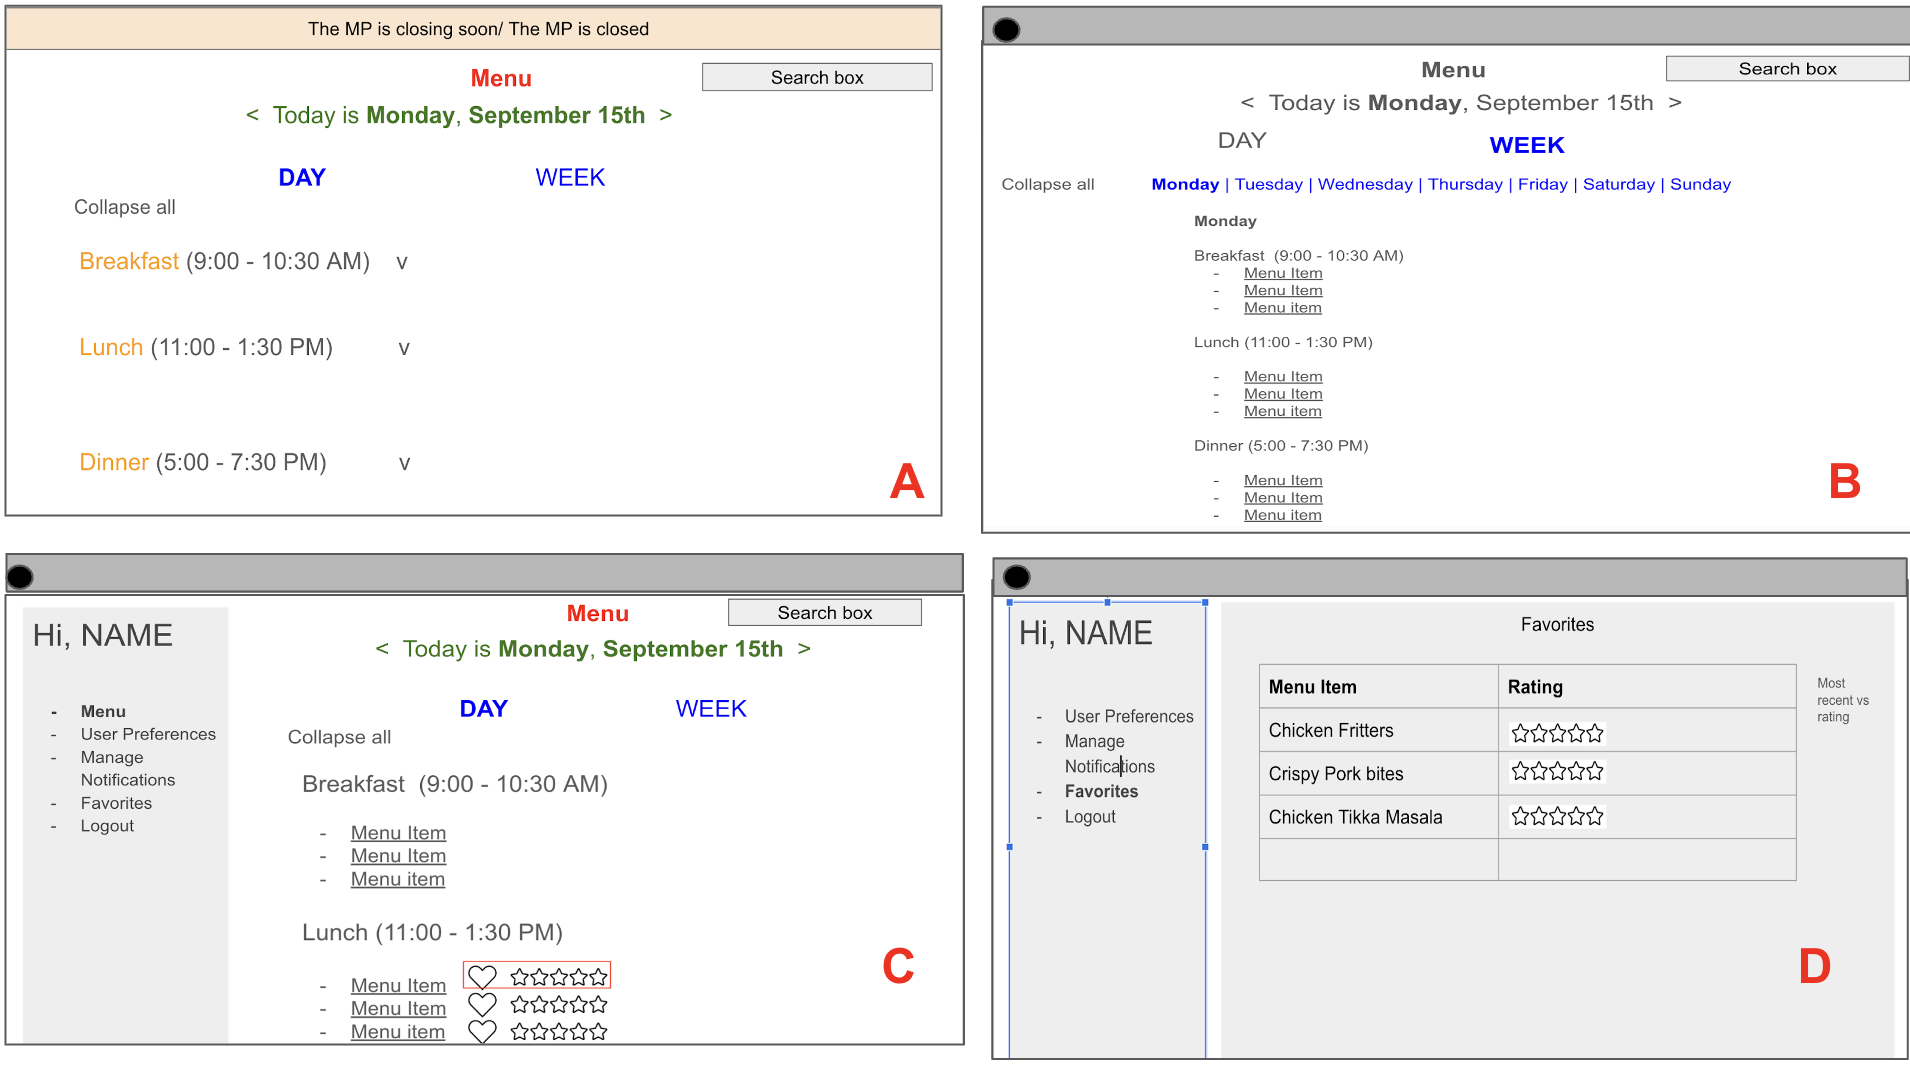
\includegraphics[width=1.0\linewidth]{images/prototype2.png} % Adjusted width
    \caption{
         Wireframe prototype of the main UI
    }\label{prototypes}
\end{figure}




In Figure.\ref{prototypes} there are labeled red letters in the bottom right of each quadrant; I'll describe each in order.

The landing page (quadrant \textbf{A}) is designed to provide a clear and intuitive overview of the day's menu, ensuring users immediately know what is being served. A placeholder logo is positioned in the upper-left corner of the page. This follows the widely accepted web design convention of placing logos in the top-left, as users intuitively look to this area first for branding and navigation cues. An admin-controlled announcement banner appears at the top of the page, ensuring visibility without overshadowing the main content. The book advises positioning urgent or important updates in prominent areas that users encounter first upon loading a webpage. Just below the banner positioned in the top-right corner is the search bar. The top-right corner is a conventional placement for search functionality in web design because it aligns with users' natural scanning patterns from left to right, as highlighted in the Web Style Guide \cite{Web2009}. The page's title (e.g., ``Menu") is displayed prominently below the banner to orient users. Below the header, a subtitle shows the current date (e.g., ``Monday, September 15th"). Interactive left and right arrows on either side allow users to navigate to the previous or next day’s menu. 

Moving onto quadrant \textbf{B}, we see the dual menu navigation. Two tabs can switch between ``DAY" and ``WEEK" views. The 'DAY' feature introduces a new navigation option for users, while the 'WEEK' retains the familiar 'jump-to' functionality from the current webpage, reflecting user feedback that appreciated this feature. The selected tab is visually highlighted for clarity. Dining periods (e.g., Breakfast, Lunch, Dinner) are displayed in collapsible sections with dropdown arrows to expand or hide menu items. Inspired by the previous studies' emphasis on ``logical grouping of related content," these tabs allow users to toggle between detailed each dining period seamlessly. Each meal title is accompanied by indicative times (e.g., ``Breakfast: 7:00 AM - 10:00 AM") to provide additional context.

Lastly, quadrant \textbf{C} and \textbf{D}. The logged-in dashboard provides enhanced functionality and personalization features for student users. A left-hand side panel offers one-click access to key features like viewing menus, rating meals, and saving favorites. The decision to include a sidebar for logged-in users  was guided by the book's emphasis on ``intuitive navigation for hierarchical content." This left-aligned navigation is standard because it allows users to quickly locate tools without excessive page scrolling, reducing cognitive load \cite{Web2009}. The active tab is visually highlighted, allowing users to track their current location easily. By displaying detailed information in a structured and intuitive way, this design supports the principle of perceivable information, ensuring all users, regardless of ability, can access and understand the data provided.

I did not formally test the prototypes but presented them to my peers in Senior Seminar. Feedback was generally neutral to positive, with no major questions or confusion about the design or element placement.

\subsubsection{Color Palette and Font}

The Web Style Guide emphasizes the importance of consistent font and color choices, as consistency in design helps users navigate the site intuitively and reinforces the brand identity \cite{Web2009}. For this project, I chose a color palette of orange, black, and white to align with Occidental College's branding and create a sense of familiarity for users. I made sure to use Oxy's signature orange (HEX color \#ff744c), which ensures consistency with the institution's identity, reinforcing trust and recognition. For font selection, I aimed for a balance between clarity and engagement. In the initial surveys and interviews, users expressed a desire for the design not to feel ``boring," and the primary goal was to ensure the font remained legible across all devices and sizes. To further support Universal Design principles, I included a dark/light mode toggle, allowing users to adjust the color scheme to their preference. This functionality accommodates users with light sensitivity and makes the interface more comfortable in different lighting conditions.

\subsection{Implementation}
With the requirements set and designs conceptualized, the implementation phase focuses on translating the prototypes into a fully functional website. I began by implementing the front-end interface, ensuring all components and modules were functional before integrating the backend. Thus, this section will discuss high-level implementation decisions and their rationale. For more detail on techniques or systems used, see the code architecture overview in Appendix \ref{Code-Arch}.

\subsubsection{Frontend}

The application's front end was developed using ReactJS to create a visually appealing, responsive interface. Mobile responsiveness was prioritized, as user interviews revealed frequent mobile use for quick menu access. Using Google Chrome's inspection tools, I tested compatibility across various iOS and Android platforms. I also ensured desktop compatibility in both Chrome and Safari when developing in my local environment. Key design features include collapsible accordion sections for daily and weekly views, dynamic creation of sections based on the dining schedule, and bold text for serving stations to improve clarity, addressing user feedback. The search functionality compensates for the lack of nutritional filtering, enabling users to find menu items by keywords like ``pasta" or ``grill." Results include the meal item, date, serving station, and meal section (e.g., Breakfast), displayed in a user-friendly modal. Inspired by the comparative analysis SCIAC menu pages, I made it so the web app also features an auto-day load function that fetches the current day's menu upon initialization, ensuring the displayed menu aligns with the date. The 'Feedback Form' is embedded as an iframe for easy student access, and admin can view responses as an embedded iframe. I decide to switch the feedback from being used as part of the database to embedded iframes to streamline access and maintain consistency with the existing Google Form system, minimizing the need for additional backend integration. In the navigation bar, the 'Traffic' dashboard shows MP activity levels, and I credited a peer’s Raspberry Pi system, linking it on the landing page to acknowledge their contribution.

\subsubsection{Backend}
The backend serves as the operational core of the application, doing “behind the scenes” work. The core part of the menu webpage is the menu; if the menu is not working, the website serves no purpose. I implemented the scraping process using Axios for HTTP requests and Cheerio for HTML parsing. Every Sunday, the scraper fetches the weekly menu from the Marketplace website, targeting specific HTML elements to extract meal data. I configured the scraper to run periodically throughout Sunday, ensuring the most accurate data was captured regardless of when the updates occurred. Once fetched, the data is compared with existing entries in the MongoDB database, and only new or modified items are written. I extensively used MongoDB’s visualizer tools during development to verify data accuracy and refine the schema.

The backend is built with Node.js, using GraphQL for data queries and MongoDB for storage. I chose GraphQL over REST APIs because its ability to handle complex queries reduced the need for multiple endpoints and simplified data retrieval for the front end. I structured the database schema to support all core functionalities of the dining system. The Menu and Meal tables organize meals by day and date, while the Rating, MenuItem, and Feedback tables track user interactions such as meal ratings, favorites, and feedback submissions. Admin-specific operations, like updating OperatingHours and Banners, are also managed within the schema. Additionally, after discussions in Senior Seminar regarding whether the menu would always be updated via the scraper, I explored options for manual updates. Consequently, I implemented an 'Add Menu Item' feature allowing admins to manually add menu items using input and dropdown fields. These items are saved in the database in the same way as those pulled by the scraper, with dietary labeling included as part of the menu item's text, ensuring consistency. In creating the backend of the 'Weekly Menu Newsletter', I automated email notifications using my own Gmail account, which was configured for secure SMTP access. I implemented a CRON scheduler that runs every Monday after the menu scraping process, automatically sending the updated weekly menu to subscribed users. This automation eliminated the need for manual intervention, ensuring timely delivery and reducing admin workload. Throughout development, I heavily relied on YouTube tutorials to navigate the challenges I encountered (such as getting started and addressing errors) while building my first full-stack backend. It was very important to watch visual tutorials because I am a visual learner. An entity relationship diagram illustrating the database schema is provided in Appendix \ref{erd} and the GitHub repository under .FinalPaper/assets. 

\subsection{Testing}

    \begin{figure}
    \centering
    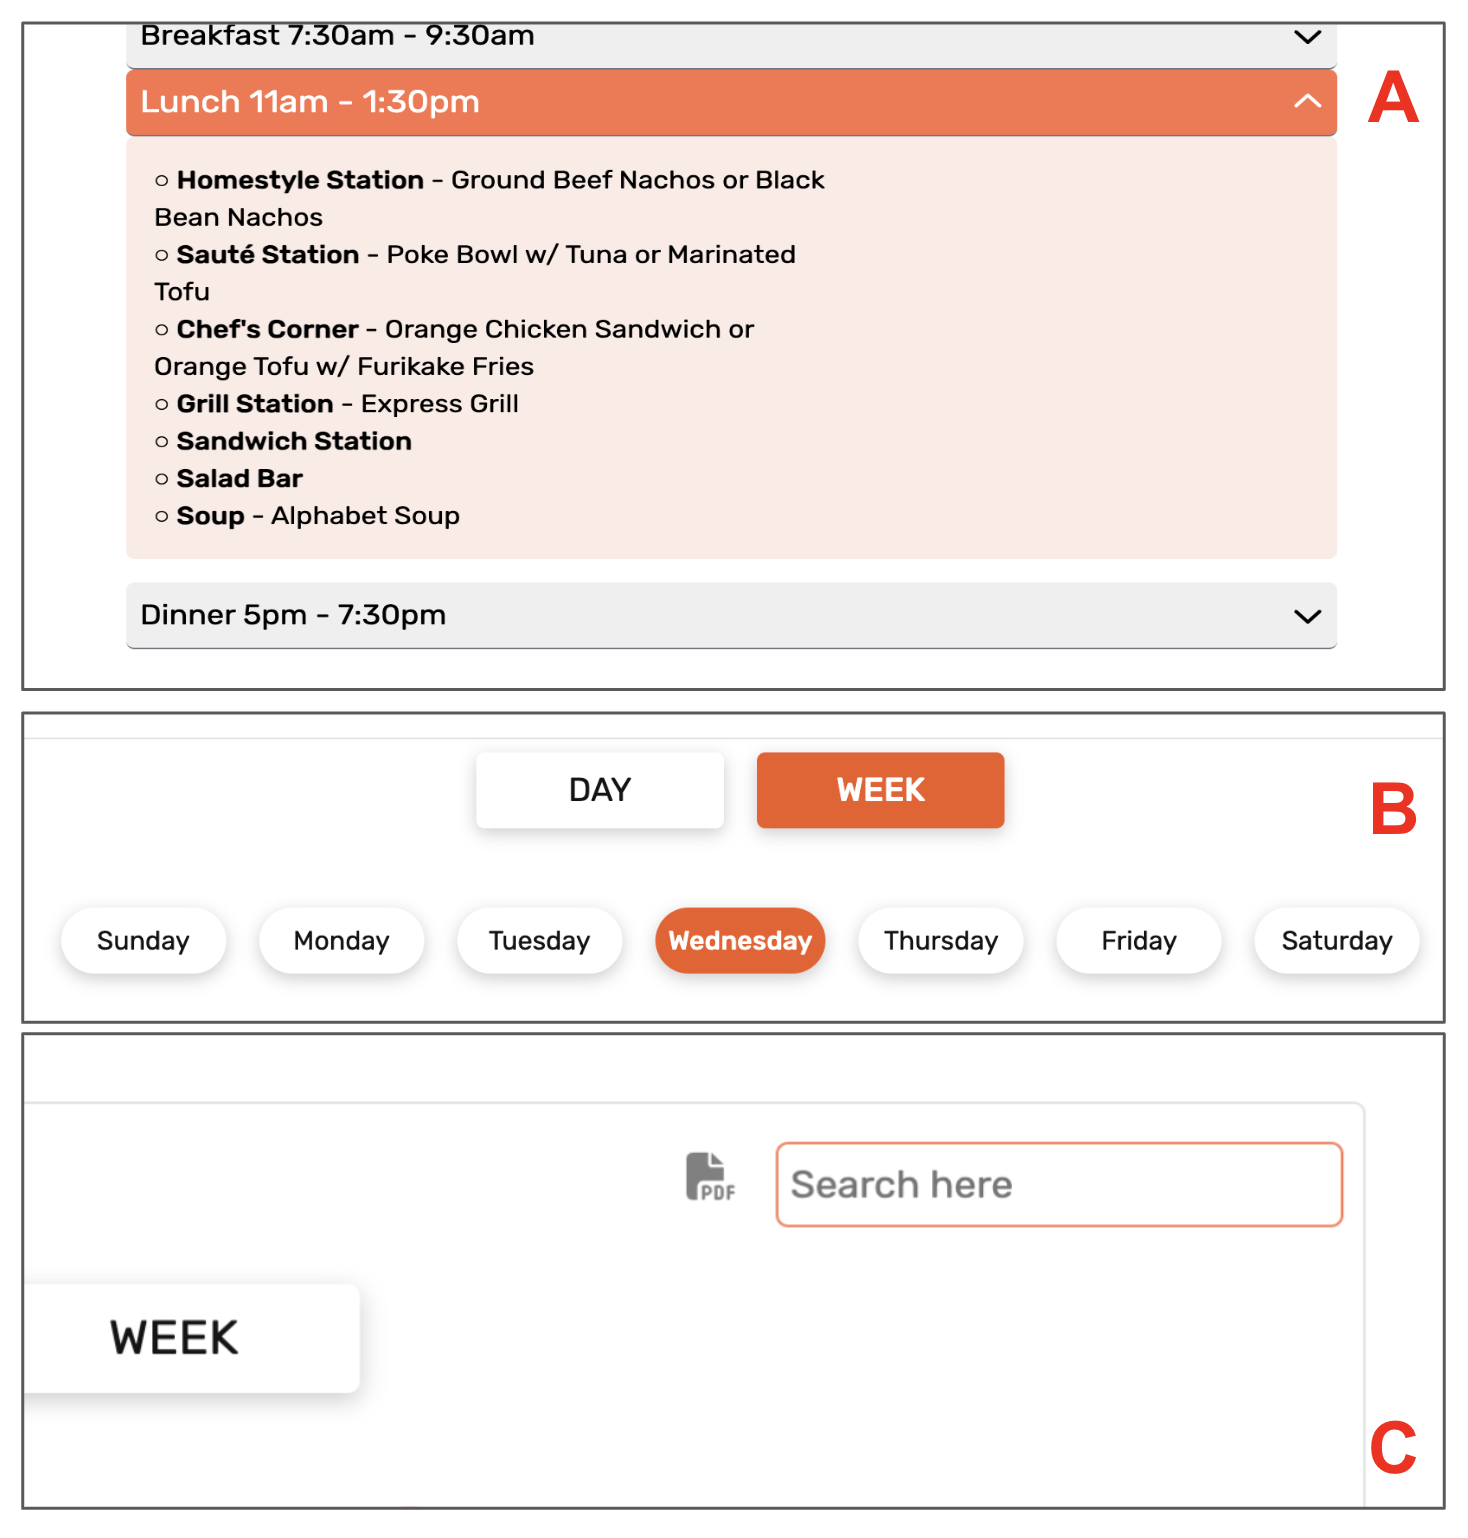
\includegraphics[width=.95\linewidth]{images/testing-Ui.png} % Adjusted width
    \caption{
        Initial UI 
    }\label{initial-UI}
\end{figure}

In informal user testing sessions with the early version of the application, users expressed generally positive reactions to the functionalities demonstrated by the application. They also appreciated the overall design and aesthetic appeal, many saying it was ``exciting" to look at. Surprisingly, many users appreciated the dark vs. light mode feature, which I initially doubted would be easily discoverable due to the subtle moon-and-star icon in the upper corner. 

Additional feedback revealed specific areas for improvement. For instance, users found the accordion/collapsibility feature of the menu sections unintuitive. When one section, such as ``Breakfast," was open, clicking on another section, like ``Lunch," automatically closed the first. This is shown in the quadrant labeled \textbf{A} in Figure. \ref{initial-UI} as lunch is open and the other components are closed. To address this, I modified the React component to manage collapsibility by replacing the single-state logic with a multi-state toggle, allowing multiple sections to remain open simultaneously. In the final UI, I added a Expand All: Collapse All text button that offers dual functionality, manually clicking a section(s) to open or being able to open all and close all with the click of one button. Additionally,  there was significant excitement for the dual menu navigation by day or by week. Two users suggested showing the date (e.g., October 14th, 2024) alongside the day in the week view when switching between days; this is shown in the quadrant labeled B in Figure. \ref{initial-UI}. I hadn’t considered this perspective but immediately recognized its value. I implemented it to improve navigation and help users see the day and its corresponding date quickly.

Another notable issue was the lack of an option to view an entire week's menu simultaneously, which a few users mentioned would help with meal planning.  Before deciding to implement this, I wondered how it would differ from pressing ``Ctrl + P" to print the current MP menu webpage which essentially does the same thing. However, this feature is much more convenient because it automatically generates a clean, pre-formatted PDF that opens in a new tab with just one click, saving users time and effort. To address this, I implemented a ``Download Weekly Menu" feature that generates a PDF of the week’s menu. The implementation was relatively uncomplicated because an intricate method already existed for fetching the menu data, which I used for generating the weekly email newsletters. Using the jspdf library, I dynamically pulled this data from the backend API, formatted it into a clean, structured layout, and generated a downloadable PDF. After implementing the feature, users noted that the generic PDF icon was not intuitive (see Figure. \ref{initial-UI}, quadrant labeled C). To resolve this, I replaced the generic icon with a more descriptive React component from the react-icons library, specifically an export download icon, to better communicate the button's purpose and improve usability. 
Another significant issue surfaced during a class presentation in a senior seminar, where I demoed the student and admin dashboards. The application experienced a 20-second delay during login, leaving the audience (and myself) uncertain if the system worked. A student suggested adding some indication that the backend was working on validating authentication to improve clarity during this process. I implemented this by adding a loading spinner that activates immediately after the user submits their credentials and a modal in the corner of the screen that provides feedback on whether the login was successful or if there was an error. This resolved the ambiguity users may experience during authentication. Feedback on the ``Busyness" tab highlighted its confusion among users, leading me to rename it ``Traffic," a concise and clear option inspired by Google’s Business Profile ``Popular (Peak) Times" feature, which maintained the navigation bar’s simplicity.
Additionally, while conducting user testing interviews with an admin staff member from the ‘Front of House team,’ I received generally positive feedback on the design and functionality, particularly the management controls. However, I noticed hesitation when they navigated the tabs. They mentioned that some tab names were unclear, leading to confusion about their functions. For example, the previously labeled ``Emails" tab was renamed ``User Details" to better indicate its purpose. At the time, I struggled to implement the backend for the rating and favoriting system to visualize the data effectively, so I chose not to demo that feature. The final UI for Admin Dashboard favorite and rating insights can be found in Appendix \ref{ratings-favorites}. 

\subsubsection{Special Use Case: No Menu Found}
During Thanksgiving break, when the MP was closed for three days, I implemented a live operating hours indicator on the frontend. Admins manage this feature by inputting opening and closing hours for each day, Sunday to Saturday. However, I noticed the scraper method lacked a fallback for days without a menu. To address this, I integrated the operating hours feature to display a clear message when no menu was available. If the MP was closed, as indicated by ``00:00" operating hours in the database, a message would inform users of the closure and prompt them to check operating hours (this text is hyperlinked to a modal, this is shown in quadrant \textbf{A} of Figure. \ref{final-UI-mobile}. This improved user clarity during holidays or closures. I also realized the need to permanently display the MP’s daily operating hours on the landing page. After testing various placements, positioning them near the export-PDF icon proved most effective, aligning with functional elements and ensuring logical flow. Differentiating the icon's color enhanced visibility and usability. The final UI adjustments, based on feedback, are shown in Figure. \ref{final-UI-desktop} (Desktop) and Figure. \ref{final-UI-mobile} (Mobile).
    \begin{figure}
    \centering
    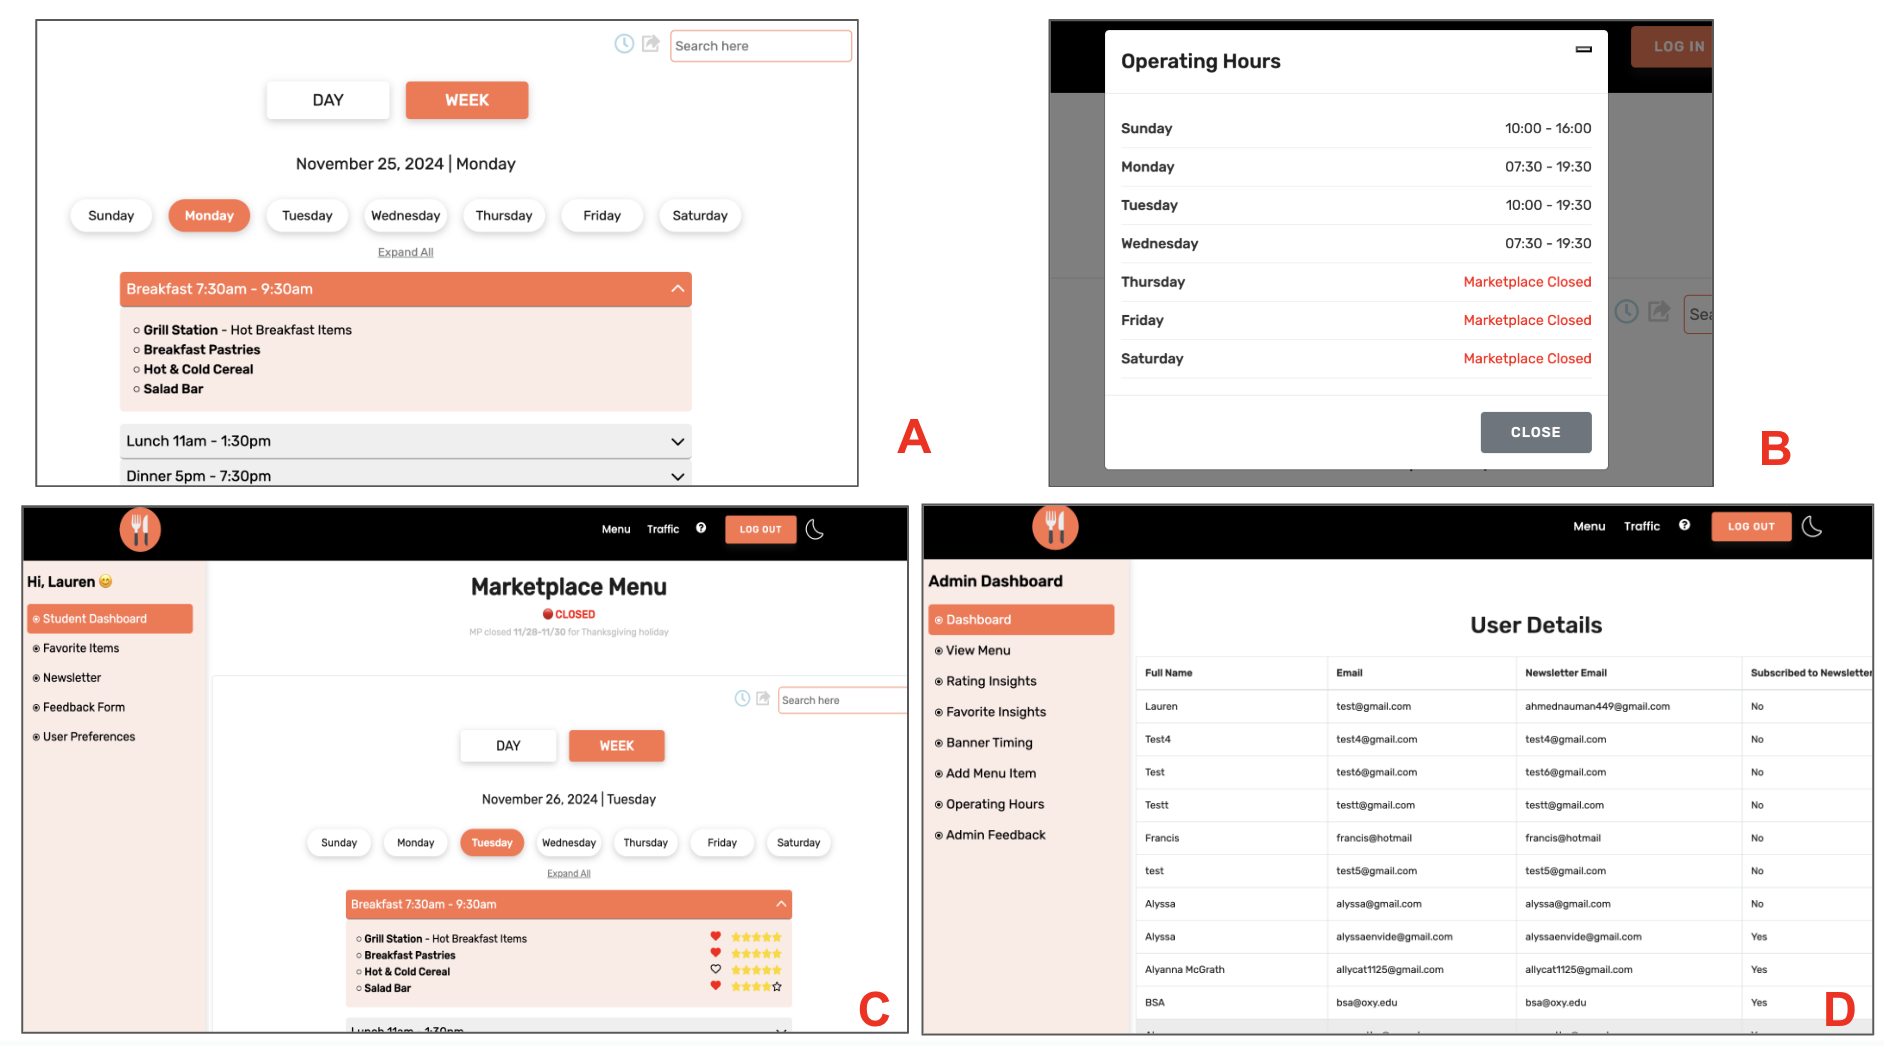
\includegraphics[width=1.0\linewidth]{images/final-UI-desktop.png} % Adjusted width
    \caption{
       Final UI for desktop: A) Landing page, B) Operating hours modal, C)Student dashboard, and D) admin dashboard.
    }\label{final-UI-desktop}
\end{figure}
\begin{figure}
    \centering
    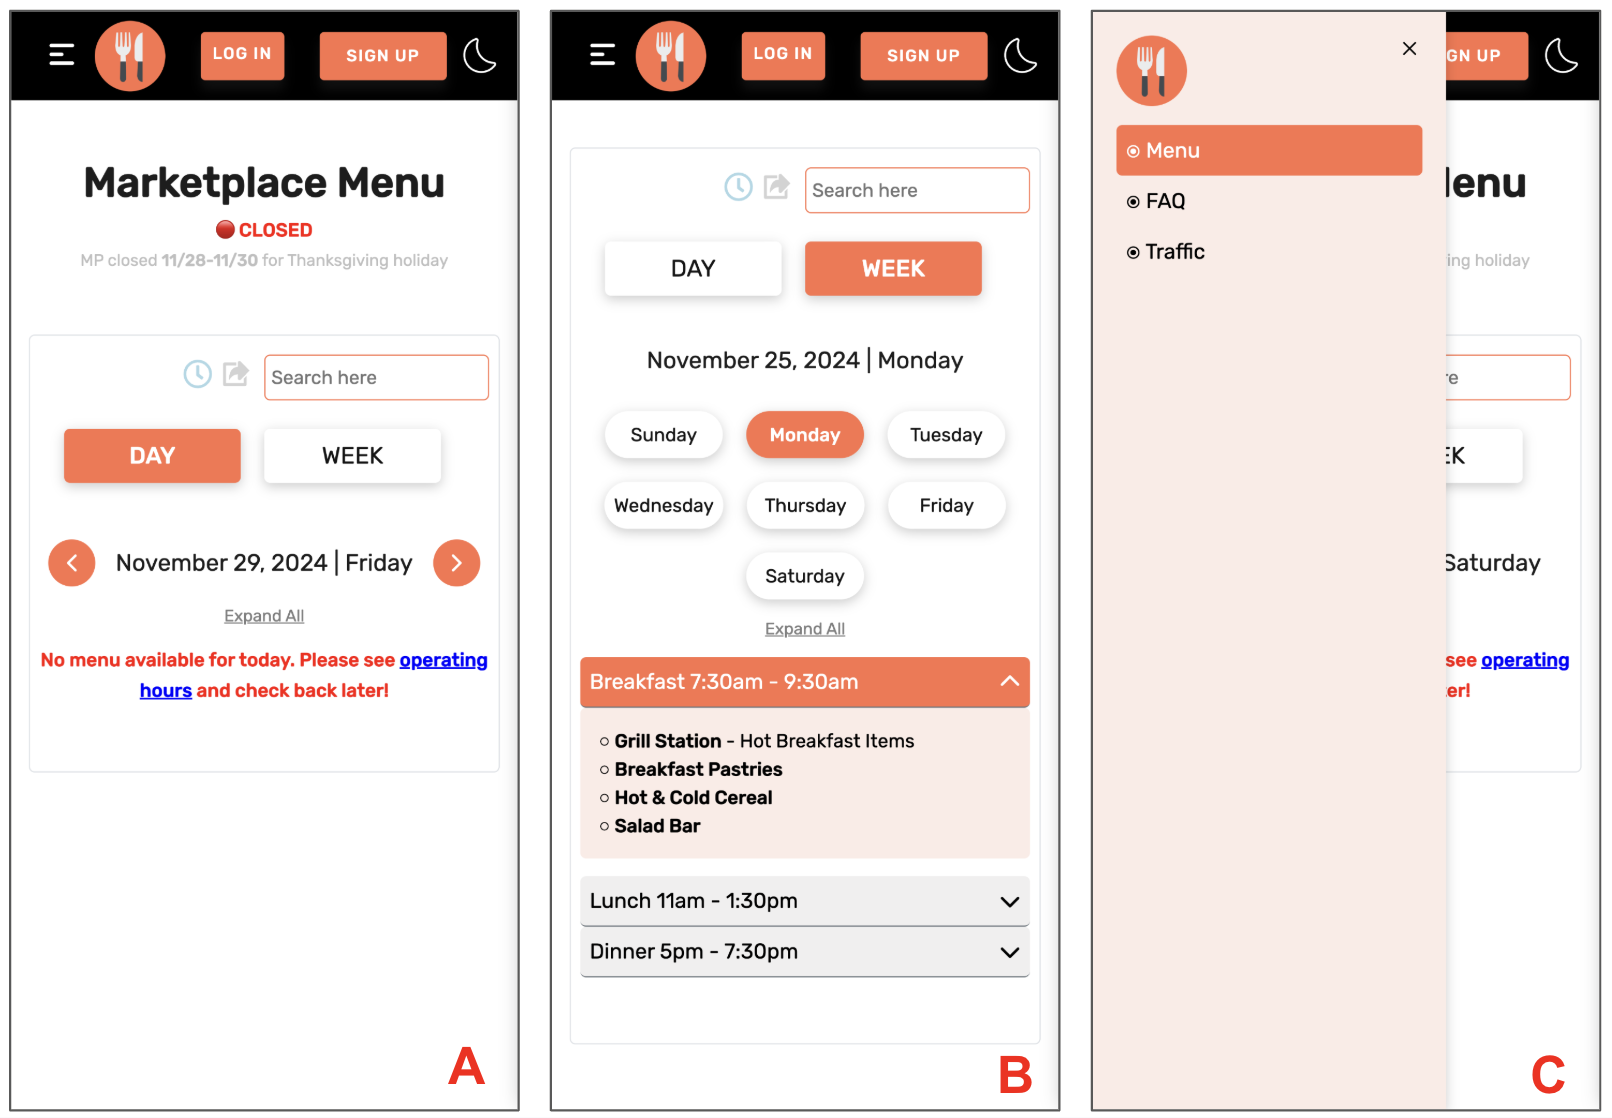
\includegraphics[width=1.0\linewidth]{images/final-UI-mobile.png} % Adjusted width
    \caption{
       Final UI for mobile: A) Landing page, B) Week view on the landing page, and C) Sidebar displayed when the hamburger menu is selected.
    }\label{final-UI-mobile}
\end{figure}

\section{Evaluation Metrics}
To evaluate the project, I conducted in-person one-on-one interviews with nine students selected from the first group of 23 who completed the initial survey during the Requirements phase. I narrowed down my user group for focused feedback while ensuring diverse perspectives. The interviews were structured into three stages: 1) a ``free-fall" phase where students explored the app without my guidance to observe their natural interactions, 2) a timed task phase to assess specific features, and finally, 3) a directed Q\&A phase focused on their experience with the web app. For the timed task phase students completed tasks on both my application and the existing MP webpage, allowing for a comparison of usability, functionality, and overall experience. I randomized the order with five students, first doing tasks on the MP webpage and the rest doing them on my application first. Later that week, students completed a final survey with 5-point Likert scale questions ranging from ``Strongly Disagree" to ``Strongly Agree" and satisfaction questions rated on a scale of 1 to 10. Additionally, I asked a Net Promoter Score (NPS) question to assess advocacy. Advocacy is the likelihood of users recommending the product or service to others. I used the NPS because it is a widely accepted metric that provides valuable insights into user satisfaction \cite{NPS}. For the administrative evaluation, I took an observational approach, providing the Director with access to the dashboard and taking detailed notes on their behaviors, comments, and feedback. During in-person interviews, my application was only accessible via my local server. I decided to deploy the web app using Cloudflare Workers before sending the final surveys out so students could interact independently, on their mobile devices and computers, and provide more meaningful feedback. At this time is when I formally named my solution OxyEats, inspired by UberEats, not only for its brevity but also because I personally liked the name. This also offered a user-friendly URL, https://oxyeats2.pages.dev/. 

To evaluate the success of my project, I will focus on two key metrics: increased usability and enhanced user experience, with separate evaluations for students and administrators. Usability will be measured by comparing task completion times, with shorter times indicating success. User experience will be assessed through Likert scale surveys and open-ended feedback for qualitative and quantitative insights. Observational interviews and surveys will gauge how well the solution meets student needs, while administrator feedback will focus on usability and workflow integration. Success will be defined by reduced task times, higher survey scores, and positive feedback, with neutral outcomes indicating minimal change and negative results signaling failure, and the need for extensive improvements.

\section{Results and Conclusion}
The final survey data for this evaluation can be found in the .FinalPaper/assets directory under 'Final User Testing Survey' \cite{GitHubRepo}.

\subsection{Usability Results}

Across nine students, two first-years, two sophomores, two juniors, and two seniors, OxyEats demonstrated faster task completion times across all scenarios. The structure of the timed task scenarios was as follows: I asked participants to complete specific tasks, starting the timer immediately after I finished describing the scenario. It is important to note that I gave students a hypothetical scenario and didn't just say to search for “Chicken” because it encouraged them to engage with the app more naturally. By framing the task within a scenario, I observed how they interacted with the app's features in a practical context rather than simply following direct instructions. The clock stopped when participants verbally indicated task completion by saying, ``I'm here" or ``done." Locating today's lunch menu averaged 1.53 seconds on OxyEats compared to 3.83 seconds on the MP webpage. Similarly, finding all menu items with the keyword ``Chicken" averaged 3.26 seconds on OxyEats, significantly outperforming the MP webpage's 7.53 seconds. As students completed these tasks, I took note of any behavioral insights. Many students instinctively relied on the auto day-load feature to locate today's menu, often realizing it was already displayed before actively searching. In contrast, on the MP webpage, they either scroll until the day or use the jump-to feature, which was still slower. This led to faster completion times and positive remarks about the app’s intuitiveness. When using the search functionality in my solution, participants appreciated the simplicity but occasionally struggled with keyword specificity, which some noted could be improved with suggestions or typo tolerance. The way results are formatted on my solution served for better efficiency as all students used command + F to search keywords on the MP menu webpage, which led to slower completion times, and often times its search mechanism was not accurate, often pulling up words that were part of other words (e.g., “rice” within “price”). In contrast, my solution's formatted search results provided a clearer and more organized experience.  

The critical takeaway from comparing navigation between my solution and the current MP solution is the efficiency of my design. In my solution, navigating between days or weeks is just one click away using the week or day view. In contrast, the MP solution requires users to manually scroll through the entire page, often overshooting the desired day due to the lack of distinguishable text formatting. This would be slightly improved  if there were a “back to top” button, but there is none.

\subsection{User Experience Results}
The user experience evaluation combined qualitative insights from post-task interviews and quantitative survey data to assess satisfaction, engagement, and functionality. The post-testing survey revealed a mean satisfaction (how satisfied are you with the overall service provided by this new solution for the MP menu webpage?) rating of 9.2/10, indicating strong overall app approval. When asked if they would use this solution for checking dining options in the future, 100\% of participants responded with”likely” or “highly/very likely” further emphasizing the app's value in their day-to-day dining decisions. The NPS was calculated based on a binary ``Yes" or ``No" question: ``Would you recommend this solution to a friend?" Since 100\% of participants answered ``Yes," the NPS score was a perfect +100. This score highlights users' strong belief in the app's ability to enhance their dining experience and make it worth recommending to others. The comparison of survey responses revealed several critical insights into the improvements in user experience provided by OxyEats. The ease of navigation also showed substantial improvement, jumping from 3.33 to 4.89. Additionally, satisfaction with text placement and formatting improved dramatically, indicating that the app’s clean and visually appealing design played a major role in enhancing user satisfaction. The full comparison table, of average responses from initial vs final survey can be found in Appendix \ref{survey-compare}. Collapsible menus and toggles were frequently praised by users for effortlessly switching between meals or days without cluttering the interface. The search functionality was another standout feature, enabling quick and efficient location of specific menu items, which users found particularly valuable.  Additionally, the ability to favorite and rate menu items was viewed as a helpful tool. However, some features were deemed less useful by participants. While dark mode was appreciated, a few users pointed out that the text contrast in this mode could be improved for better readability on mobile devices. The newsletter subscription feature was considered unnecessary, as users were generally uninterested in adding another email to their already overflowing inboxes. Some users perceived the option to download menus as PDFs as unintuitive or unclear in its purpose. Behaviorally, many users expressed confusion, often commenting, ``Oh, what does this do?" or ``What is this for?"

\subsection{Admin Evaluation Results}
While developing OxyEats, I planned to meet with Director Martinez and the front-of-house manager who oversees the menu webpage. However, due to scheduling conflicts and overlapping vacations, I could only meet with Martinez, who oversees the entire dining operation. In hindsight, I should have planned more proactively to capture additional insights on how the solution could address the front-of-house team’s challenges and opportunities.

In our final sit down Martinez found the OxyEats app highly promising and aligned with the dining department's needs. He praised its user-friendly interface, calling it ``exciting" and far more intuitive than existing systems. Features like banner messaging and the operating status system stood out for their potential to enhance communication with students by integrating announcements directly into a regularly used platform. He also valued the ability to consolidate student ratings and favorites into a dynamic dashboard, allowing for visual graphs or filtered tables to better understand preferences and adjust menu offerings. However, Martinez identified logistical challenges with implementation, including IT network and administrative approvals needed to integrate OxyEats into the dining ecosystem. He noted delays in coordinating with IT, security, and other departments at small colleges like Occidental, stating, ``It takes a very long time to get everyone on the same page." He also expressed doubts about student engagement, saying, ``I’m not sure how many students are actually looking at the menu ahead of time," based on similar systems at USC, where feedback often proved unhelpful. Additionally, he noted the lack of integration with existing platforms like CBORD and the POS system as a significant bottleneck requiring resolution for seamless functionality.

\subsection{Conclusion}
Despite some of the shortcomings discussed, I believe the project successfully achieved its primary objective of enhancing the student dining experience by significantly improving usability and overall user satisfaction. My main goal was for students to have an equally pleasurable and convenient experience in planning/preparing for the most important activity throughout the day: eating. From user testing to final evaluations, it became clear that students enjoyed the new system and could use it more effectively and efficiently. The perfect Net Promoter Score (+100) further reflects strong student advocacy, reinforcing the app’s role as a valuable tool for their daily dining decisions. Overall, the project succeeded in providing a better dining experience for students, validating the app’s core design principles. In addition to the improvements already mentioned, the main change necessary for this application to be implemented in the Dining department would be to investigate further solutions to challenges such as IT approvals, integration with existing systems like CBOARD, and concerns about the practicality of the rating system. Additionally, skepticism about whether students would proactively engage with menu tools highlights a cultural challenge not fully addressed during development. Therefore, I evaluate OxyEats as neutral in success on the Admin side. Meeting with both Martinez and the front-of-house manager would have provided a more comprehensive understanding of operational workflows, potentially uncovering additional opportunities for improvement.  

\section{Ethical Considerations}
On the surface, a web application for a dining hall menu might seem free from ethical concerns, risks, and potential harm to users. However, this is far from the truth. As a developer of OxyEats, I must be mindful of the content prioritized and subsequently relay to users.

\subsection{Data Privacy}
As the web app includes features that require users to create accounts, it introduces risks associated with data management. According to a report from Pennsylvania State University, universities, and colleges are prime targets for email scammers because many have massive, open directories of emails and are home to thousands of traditional-aged college students who may lack the knowledge of more experienced email users to spot scams \cite{Ford2023}. Thus, it increases the risk of data breaches that could compromise student information. Additionally, the sustainability and maintenance of the web app pose significant ethical challenges. Without a dedicated maintenance team or a clear succession plan, the app's continuity will become uncertain after I leave Oxy and shift my focus to my professional career. I will create detailed documentation outlining the app's architecture, user workflows, and data management protocols to mitigate these risks. This documentation will serve as a guide for any future developers or administrators tasked with maintaining the platform, ensuring a smoother transition and reducing the potential for system vulnerabilities. Future developers should prioritize replacing the current authentication system, such as Redux, with Google SSO as the first step toward enhancing security. This change would not only significantly improve the platform’s security but also streamline the login process, aligning with Oxy's existing systems managed through Google SSO and Microsoft MFA, which are already used on platforms like Canvas and myOxy.edu. This integration ensures a safer and more consistent user experience.

\subsection{Technological Solutionism}
The project also faces ethical challenges related to technological equity. The assumption that all students possess or have access to capable devices to view OxyEats is fundamentally flawed and reflects a broader issue of technological inequality. According to Gonzalez and Lynch, approximately 20\% of students face significant barriers to maintaining effective technology, such as outdated devices or unreliable internet, which can impede their academic and daily activities \cite{Gonzales2020}. This disparity raises serious ethical questions about the fairness of deploying a web-based application that not all students can utilize equally. In addition, power and computer science are tightly connected; technology is nearly ubiquitous in our world, and there is already a large power difference between those who have access to the internet and those who do not. The more effective my application is, the more I will contribute to that power difference. To tackle this issue ethically, the web app integrates alternative access methods and support initiatives that help bridge the digital divide among students, ensuring that
all can benefit from the web application. One way this is done is by ensuring that the web application is fully optimized for mobile use, as many students may not own a computer but will likely have access to a smartphone \cite{Wang2023}. In addition, incorporating basic offline features into the application proves highly beneficial. For instance, allowing students to download the weekly menu when they have internet access and then access it offline can alleviate the need for a continuous internet connection.

\section{Appendix}
\appendix

\section
{SCIAC Comparative Analysis} \label{appendix-test}
\begin{figure}[H]
    \centering
    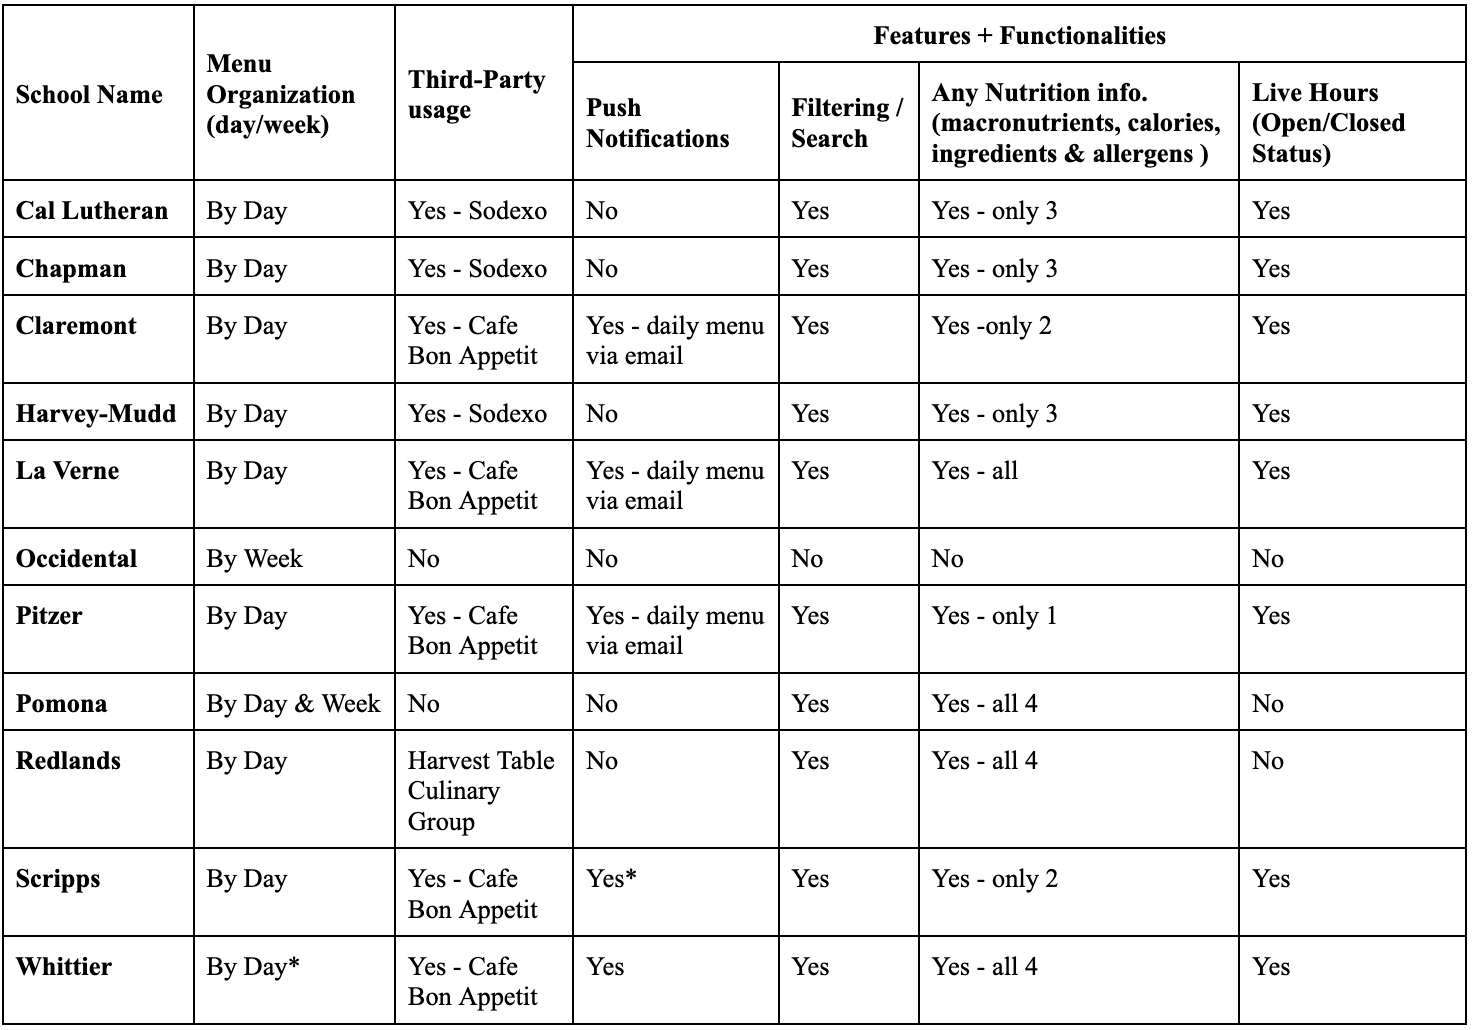
\includegraphics[width=.95\linewidth]{images/sciac-compare.png} % Adjusted width
    \caption{
        SCIAC institutions comparative analysis based on features and functionality 
    }\label{sciac-compare}
\end{figure}
\section{Waterfall SDLC} \label{waterfall-sldc}
\begin{figure}[H]
    \centering
    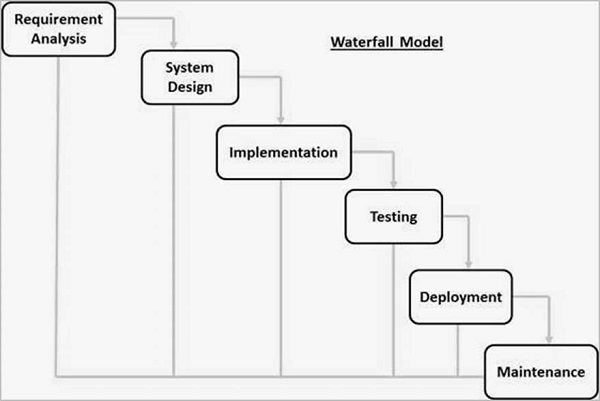
\includegraphics[width=.95\linewidth]{images/sdlc_waterfall_model.jpg} % Adjusted width
    \caption{
        Visualization of waterfall SDLC model
    }
\end{figure}
\section{Interface for Ratings and Favorites} \label{ratings-favorites}
\begin{figure}[H]
    \centering
    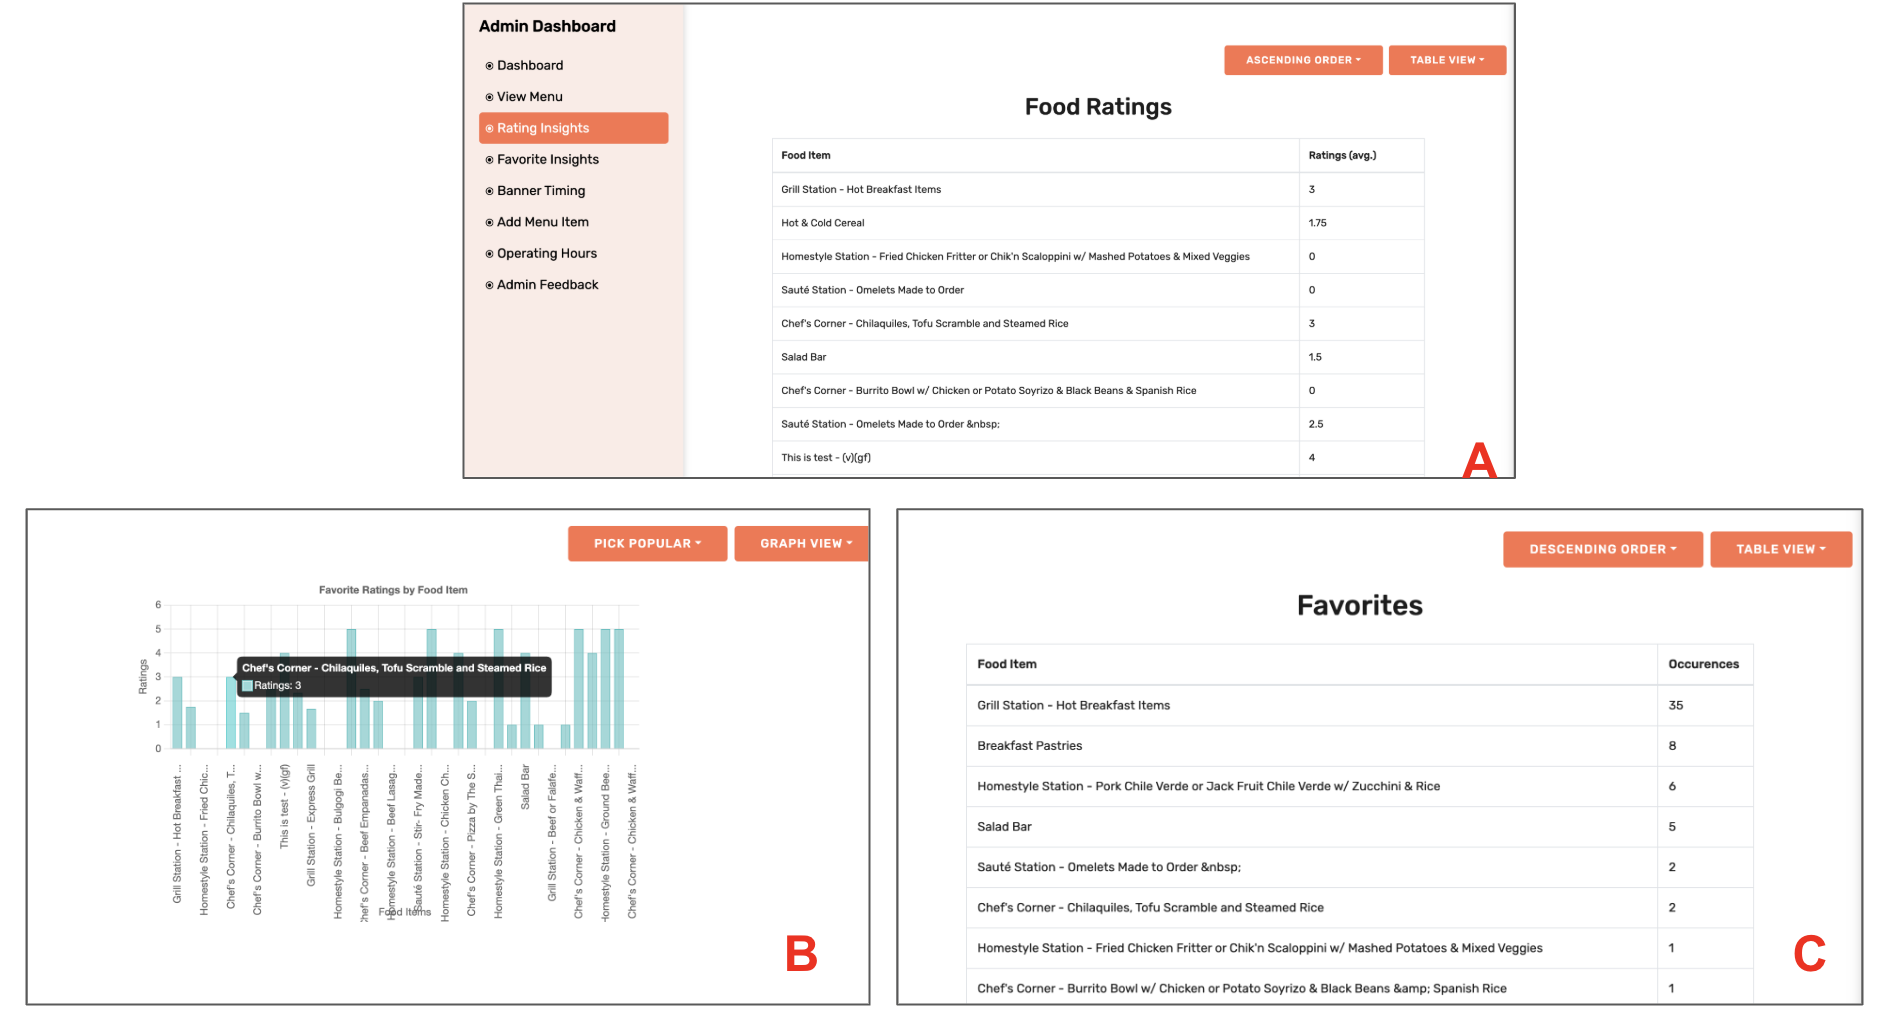
\includegraphics[width=1.\linewidth]{images/ratings-favorites.png} % Adjusted width
    \caption{
      Interface showcasing the ``Rating" and ``Favorite Insights" tabs in the admin dashboard view: (A) Ratings displayed in a tabular format, (B) Food ratings visualized as a graph, and (C) Favorites presented in a table.
    } 
\end{figure}

\section{Comparison of Avg. Survey Responses }\label{survey-compare}
\begin{figure}[H]
    \centering
    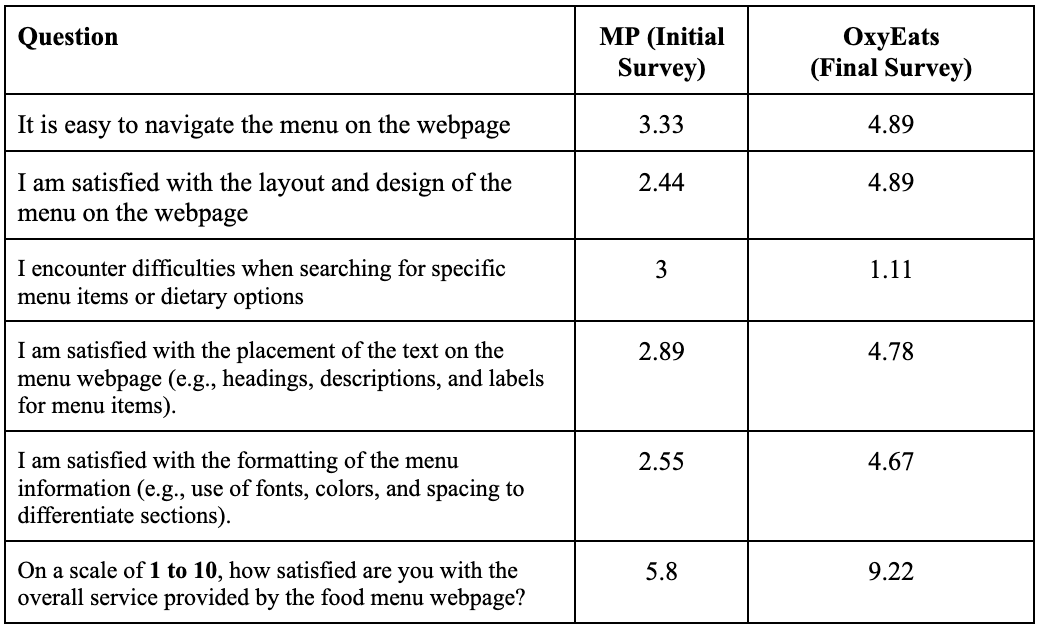
\includegraphics[width=1.\linewidth]{images/survey-compare2.png} % Adjusted width
    \caption{
        Based on a subset of 9 participants, I compared their initial survey responses about the MP webpage to their final survey responses on my new solution using a Likert scale (1 = Strongly Disagree, 5 = Strongly Agree)
    } 
\end{figure}

\section{Replication Instructions}
This section provides instructions on how to view and run OxyEats locally on your machine. The project includes a backend server and a frontend application.

\subsection{Prerequisites}
Before starting, ensure you have the following software installed (direct links to the page for downloading or installment are hyperlinked for each dependency):
\begin{enumerate}
    \item \textbf{Node.js}: v18.16.1 \textit{*Note}: npm-the package manager, is automatically included with the node.js download; I am using npm v10.9.0. Download Node.js here \url{https://nodejs.org/en} 
    \item \textbf{MongoDB}: v8.0.1 or later for the database. Install MongoDB \url{https://www.mongodb.com/docs/manual/installation/} 
    \item \textbf{Git}: to clone the repository. Install Git: \url{https://git-scm.com/downloads}
    \item \textbf{VS Code}: Editor for replication; I used this when developing a project, and the steps hereafter will refer to that. Download VSCode: \url{https://code.visualstudio.com/download}
\end{enumerate}
\subsection{Cloning the Repo}
\begin{enumerate}
    \item First, clone this repo on your local machine.:
\begin{lstlisting}[language=bash]
  % git clone https://github.com/mcgrath-a/oxyEats2.git
\end{lstlisting}
\item The code for the application is in the oxyEats2 directory. All subsequent command line instructions will be executed relative to that directory.
\begin{lstlisting}[language=bash]
  % cd oxyEats2
\end{lstlisting}
\end{enumerate}
For all the instructions below, use the integrated terminal (located in menu bar) in VS Code, which can be accessed directly within the editor.
\subsection{Setup Backend }
\begin{enumerate}
    \item In Navigate to the backend directory:
\begin{lstlisting}[language=bash]
  % cd backend 
\end{lstlisting}
\item Install all packages listed in \texttt{package.json}, run the command:
\begin{lstlisting}[language=bash]
  % npm install
\end{lstlisting} 
\textit{*Note}: If your terminal returns warnings about dependencies, run:
\begin{lstlisting}[language=bash] 
 % npm audit fix
\end{lstlisting}This should resolve any warnings and ensure your dependencies are up to date and secure.

\item Run the backend server:
\begin{lstlisting}[language=bash]
  % npm start
\end{lstlisting}
If everything is set up correctly, your terminal should display:
\begin{lstlisting}[language=bash]
    MongoDB connection successful
    Server running on http://localhost:5003
\end{lstlisting}
\textit{*Note}: If your terminal returns an error similar to the following:  
\begin{lstlisting}[language=bash]
Error: listen EADDRINUSE: address already in use :::5003
\end{lstlisting}  
this means the port `5003` is already in use. To resolve this issue, go into the configuration file \texttt{(oxyEats2/backend/server.js)} and change the local server port to an available one.
\end{enumerate}
\subsection{Frontend Setup}
Open a new terminal window, keep the terminal running the backend server open, and proceed to set up the frontend.
\begin{enumerate}
    \item Navigate to frontend directory
    \begin{lstlisting}[language=bash]
  % cd frontend
\end{lstlisting}
\item Install all React and frontend dependencies, run:
\begin{lstlisting}[language=bash]
  % npm install
\end{lstlisting}
\item Start the Client:
\begin{lstlisting}[language=bash]
  % npm run dev
\end{lstlisting}
This will start the frontend, and you should now be able to visit and use the app in browser http://localhost:5173!


\end{enumerate}
\subsection{Configuring the .env File}
The backend server relies on environment variables for sensitive configurations, such as the database connection. By default, the included `.env` file is configured for local development. \textit{However, if you want to use a cloud database like MongoDB Atlas or specify a custom MongoDB URI, follow these steps}:
\subsubsection{Using MongoDB Atlas}
\begin{enumerate}
    \item \hyperlink{https://www.mongodb.com/lp/cloud/atlas/try4-reg?utm_source=google&utm_campaign=search_gs_pl_evergreen_atlas_core-high-int_prosp-brand_gic-null_amers-us_ps-all_desktop_eng_lead&utm_term=mongodb\%20atlas&utm_medium=cpc_paid_search&utm_ad=e&utm_ad_campaign_id=19609124046&adgroup=145188748043&cq_cmp=19609124046&gad_source=1&gclid=Cj0KCQiAu8W6BhC-ARIsACEQoDCQRPEQbJ31DNbgJoK7RymGNc-6ZWI_bCXRAjLAmedXJM_Tcamwzo0aAiiQEALw_wcB}{Log in}  to your MongoDB Atlas account or create a new account. 
    \item Create a new cluster and database in MongoDB Atlas.
\textit{Steps (3-5) Obtain your MongoDB URI:}
        \item Go to your MongoDB Atlas dashboard.
        \item Select the cluster and click ``Connect".
        \item Choose ``Connect your application" and copy the provided URI.
        \item Replace `<username>`, `<password>`, and `<dbname>` in the URI with your MongoDB username, password, and database name.
    \item Update the `.env` file in the `backend` directory:
\item Save the changes to the `.env` file.
\end{enumerate}

\subsubsection{Using a Custom MongoDB URI}
If you are hosting MongoDB locally or using another MongoDB host, replace the `MONGO\_URI` value in the `.env` file with your custom URI.

\subsubsection{Testing the Connection}
After updating the `.env` file, restart the backend server:
\begin{lstlisting}[language=bash]
    % npm start
\end{lstlisting}
The terminal should display:
\begin{lstlisting}[language=bash]
    MongoDB connection successful
    Server running on http://localhost:5003
\end{lstlisting}

\subsection{Future Proofing Notes }
I've included some notes and recommendations to ensure the project remains adaptable and maintainable over time

\begin{itemize}
    \item \textbf{Dependency Management:} Use the \texttt{package-lock.json} file to lock down exact dependency versions and prevent unexpected issues caused by updates.
    \item \textbf{Containerization:} Consider implementing Docker \url{https://www.docker.com/get-started/} for streamlined replication and deployment. This approach ensures consistency across different environments by encapsulating all dependencies and configurations.
    \item \textbf{Documentation Maintenance:} Regularly update these replication instructions to reflect any changes in dependencies, configurations, or project structure. This ensures future contributors or replicators can follow the instructions without confusion.
\end{itemize}
\section{Code Architecture Overview} \label{Code-Arch}

The repository is split into two main components:
\begin{enumerate}
    \item \textbf{Frontend}: Contains the client-side code for the application
    \item \textbf{Backend}: Contains the server-side code, API resolvers, models, and utilities.
\end{enumerate}
\subsection{Key Directories and Files}
\textbf{Backend}
\begin{itemize}
    \item \texttt{graphql/resolvers}: Contains business logic for various functionalities like authentication, menu, ratings, and feedback.
    \item \texttt{models}: Defines schemas for entities such as menu, feedback, and user.
\end{itemize}
\textbf{Frontend}
\begin{itemize}
    \item \texttt{src/pages}: Encapsulates different UI pages such as home, admin, and banner.
    \item \texttt{src/components/global}: Reusable UI components like navbar, sidebar, and modals.
    \item \texttt{src/APIs}: Encapsulates API calls for specific backend interactions, keeping the data-fetching logic independent of the UI, making it easier to test and maintain.
    \item \texttt{store}: Manages application state using Redux slices for credentials, menu, and sidebar tabs.
\end{itemize}
This separation ensures high modularity and reusability, facilitating future potential for multiple developer collaboration and reducing coupling between application layers.
\subsubsection{Code Diagram}
The following figure illustrates the directory structure of the \texttt{oxyEats2} project. It highlights the organization of \textbf{key} (not all) files and directories within both the backend and frontend, showcasing their roles and relationships. 
\begin{figure}[H]
    \centering
    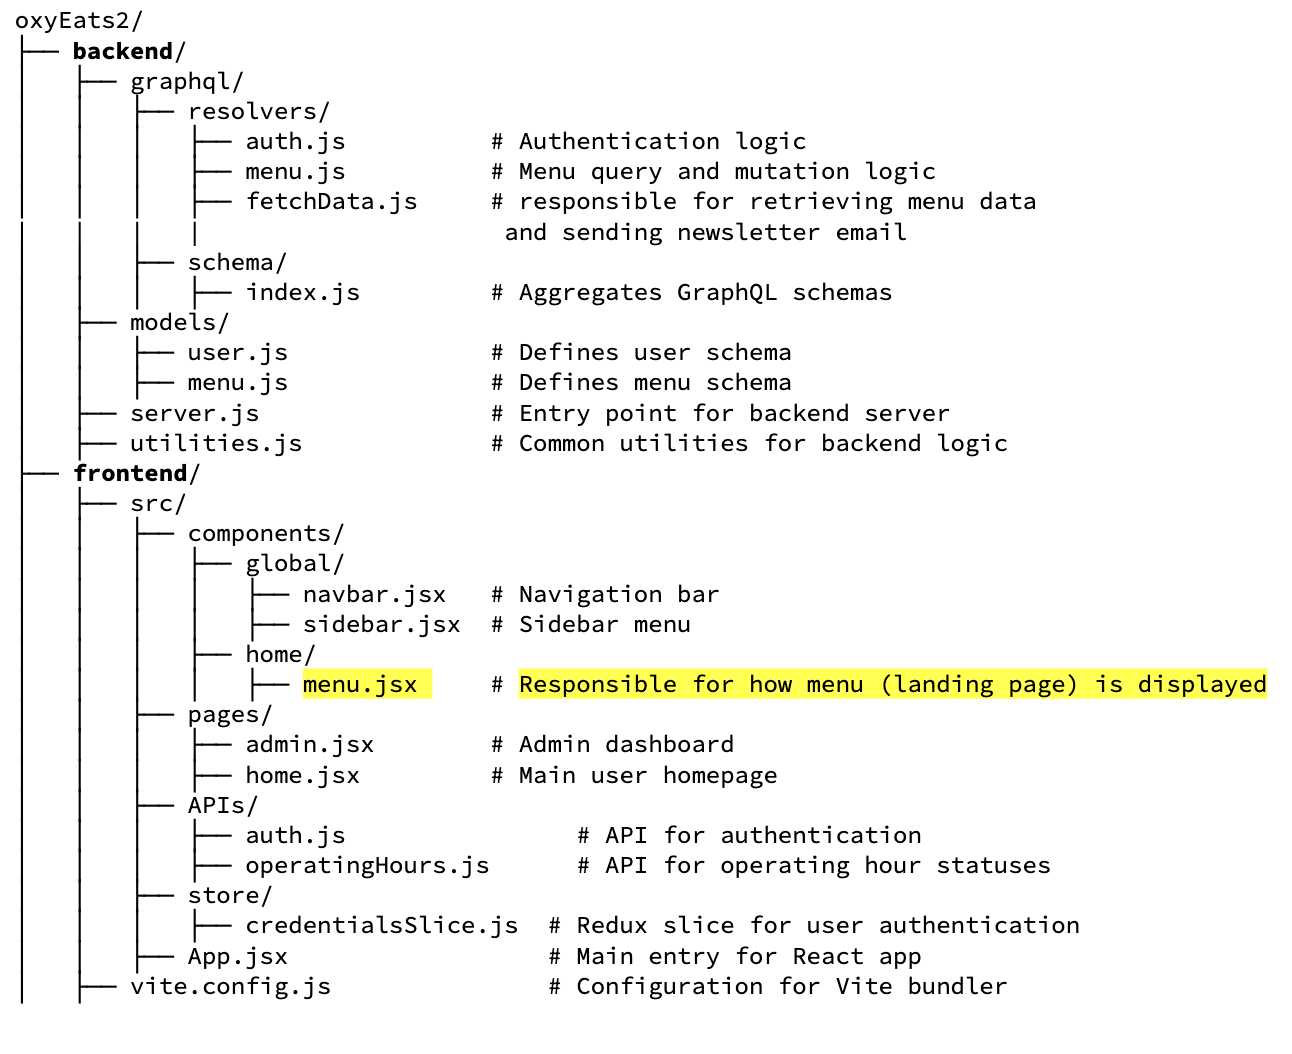
\includegraphics[width=.95\linewidth]{images/Screenshot 2024-12-05 at 4.49.59 PM.png} % Adjusted width
\end{figure}
\textbf{**Note the highlight over menu.jsx}: This component, a critical part of OxyEats, is responsible for rendering the menu page, which serves as the landing page for all users. It fetches menu data from the backend, formats it, and displays it in a user-friendly layout. The component controls the UI for displaying the operating status, exporting the menu as a PDF, managing the operating hours modal, and providing a search bar for filtering menu items. Once a user is logged in, it enables functionalities like favoriting menu items and submitting ratings.
\subsection{Database Schema: Entity-Relationship Diagram (ERD)}\label{erd}
The first diagram illustrates how users interact with other entities such as feedback, ratings, favorites and how the menu is stored within the DB, categorized by meal times (e.g., Breakfast, Lunch, and Dinner), with each meal containing a list of food items grouped by stations or themes.
\begin{figure}[H]
    \centering
    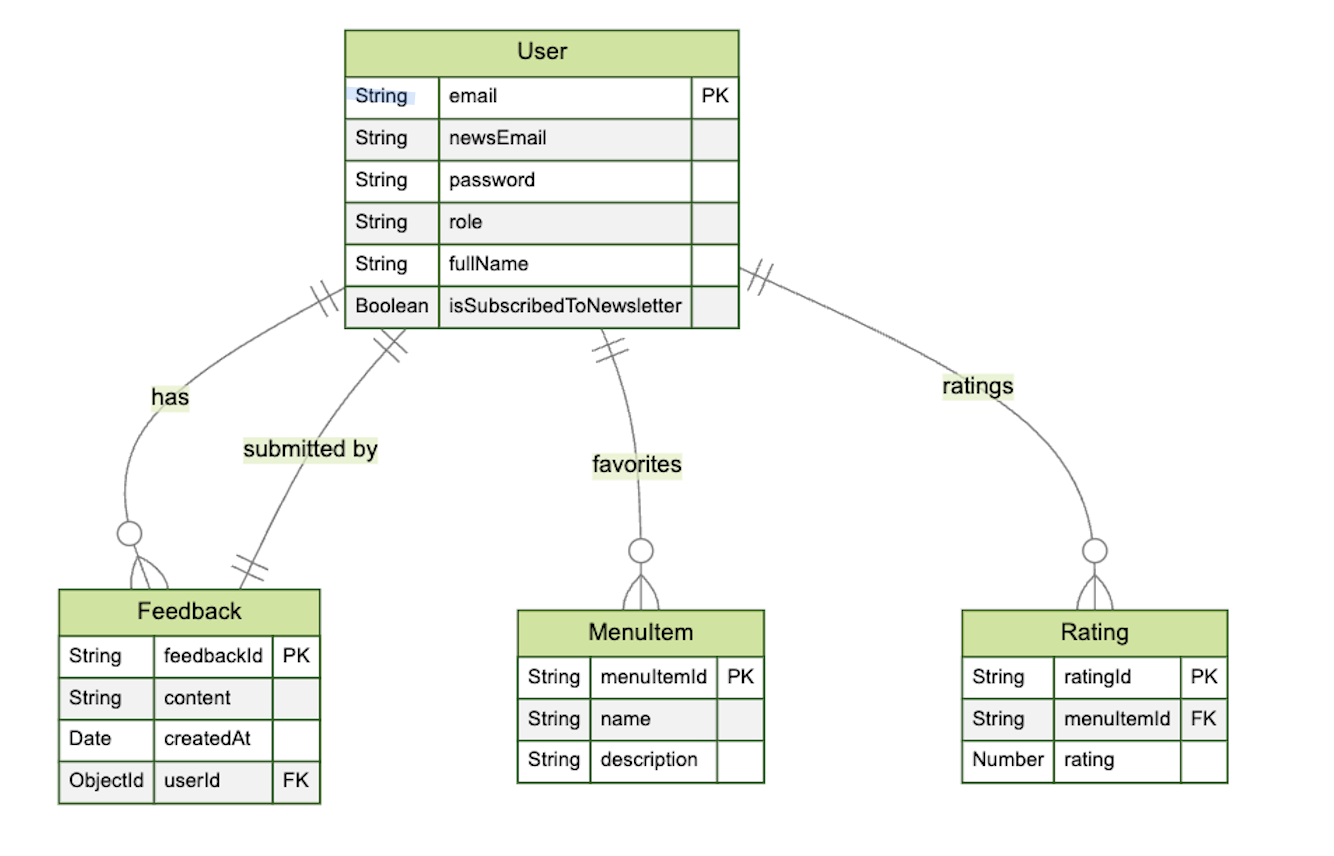
\includegraphics[width=.95\linewidth]{images/Screenshot 2024-12-05 at 4.00.11 PM.png} % Adjusted width
\end{figure}
The second diagram focuses on the administrative structure, the fetching and posting of menus, and operational elements.
\begin{figure}[H]
    \centering
    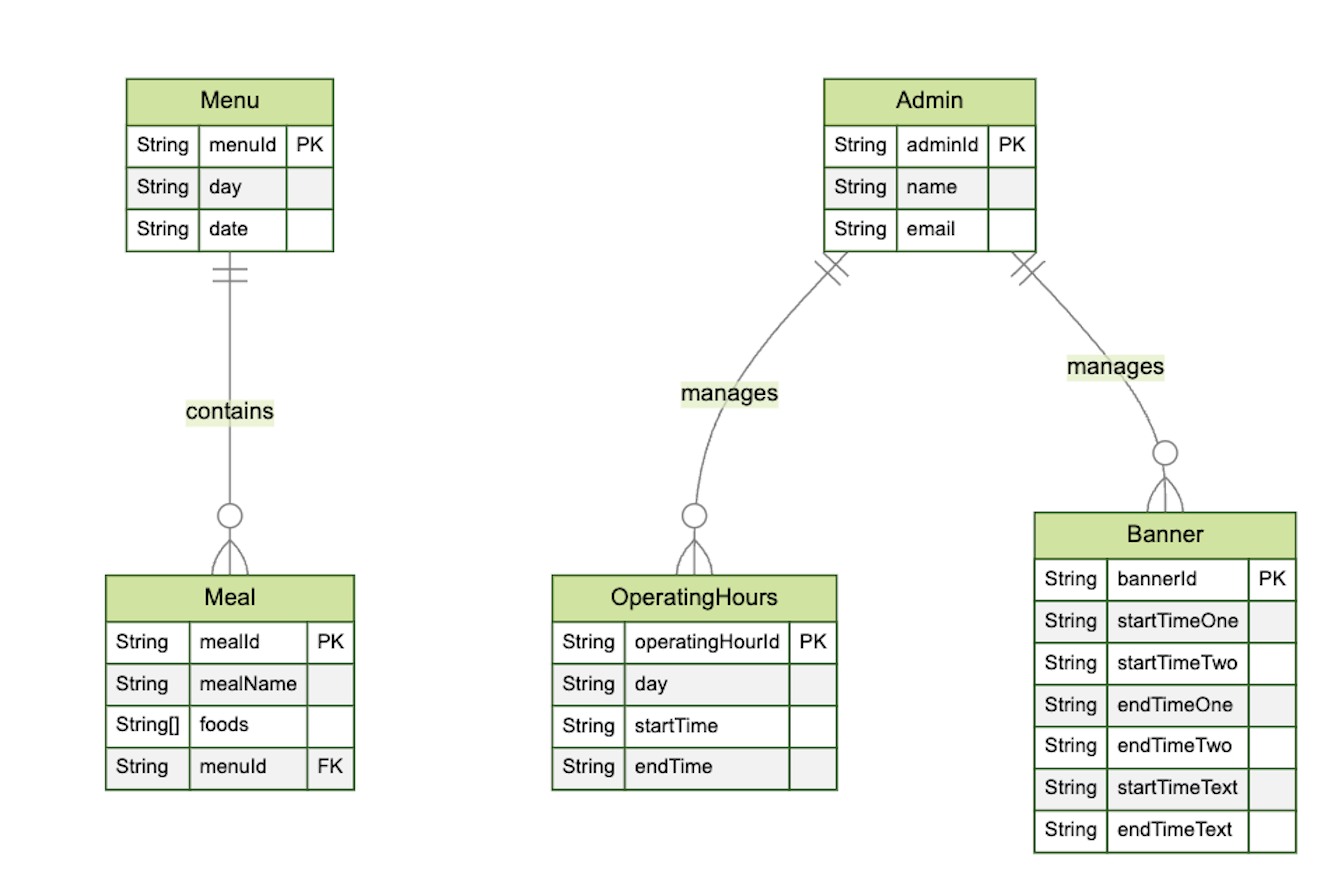
\includegraphics[width=.95\linewidth]{images/Screenshot 2024-12-05 at 4.00.16 PM.png} % Adjusted width
\end{figure}

\subsection{GraphQL}
GraphQL serves as the intermediary between the frontend and backend, allowing structured interaction with the database schema depicted in the entity-relationship diagrams (ERDs). Each entity (e.g., User, Menu, Feedback, etc.) in the database has a corresponding type definition in the GraphQL schema.

\subsection{Extending the Project}
Finally, if you wish to pick up the project the below describes what areas of the directory you should look to for what,
\begin{enumerate}
    \item \textbf{Adding Features}
    \begin{itemize}
        \item \textbf{Backend}:
        \begin{itemize}
        \item Add a new resolver in \texttt{backend/graphql/resolvers}for additional GraphQL queries or mutations.
        \item Define corresponding database schema in \texttt{backend/models}.
        \end{itemize}
        \item \textbf{Frontend}:
        \begin{itemize}
            \item Create new components in \texttt{frontend/src/components} for modular UI updates.
            \item Add new routes in \texttt{frontend/src/pages} to link the new features.
            \item Extend Redux slices in \texttt{frontend/src/store} for managing state related to new features.
        \end{itemize}
    \end{itemize}
    \item \textbf{Modifying APIs}
    \begin{itemize}
        \item Extend GraphQL schemas in \texttt{backend/graphql/schema} for new query or mutation definitions.
        \item Update corresponding resolvers in \texttt{backend/graphql/resolvers}.
    \end{itemize}
    \item \textbf{Styling Enhancements}
    \begin{itemize}
        \item Update CSS styles in \texttt{frontend/public/css} to customize the UI.
    \end{itemize}
\end{enumerate}

\subsection{Deployment Information}

The deployment strategy for the \textbf{OxyEats} project leverages \textbf{Render} for hosting the backend and \textbf{Cloudflare} for serving the entire project. 
\begin{itemize}
    \item The backend deployment on \textbf{Render} is supported by the files and configurations in the \texttt{backend/} directory, such as \texttt{server.js} (entry point) and \texttt{.env} for environment variables like \texttt{MONGO\_URI} and \texttt{PORT}.
    \item The frontend deployment on \textbf{Cloudflare Pages} relies on the \texttt{vite.config.js} file in the \texttt{frontend/} directory for build configurations, as well as the output files generated in the \texttt{dist/} folder after building the project.
\end{itemize}

\subsubsection{Advantages of Deployment Strategy}

\begin{itemize}
    \item \textbf{Fast Load Times}: Cloudflare's CDN ensures the frontend loads quickly regardless of the user's location. Render provides fast backend responses, especially when using its auto-scaling features.
    \item \textbf{High Availability}: Cloudflare and Render both offer high uptime guarantees, ensuring the application remains accessible to users.
    \item \textbf{Security}: Cloudflare's DDoS protection and HTTPS ensure the frontend is secure, while Render's managed hosting minimizes risks of server misconfiguration.
\end{itemize}

\section{Acknowledgments}
I would like to acknowledge and give my warmest thanks to my advisor, Professor Teddy Pozo, who was crucial in the conception of this project and contributed significantly with their brilliant feedback. I would also like to thank Professor Justin Li for his candid and critical comments throughout our discourse this semester; because of this, I was able to critically examine my project and paper from a new perspective, such that I am immensely proud of the end product. I would also like to thank my 'mentor' Professor Gretchen North, who has seen me grow since First Year Seminar in Spring '22. Her support and guidance carried me through to the finish line. Finally, I would like to thank my mother for everything and more. As an Engineer, you've inspired me to go into Computer Science, and I only dream of being half the person you are. Thank you all!

\printbibliography
\end{document}
